% Nejprve uvedeme tridu dokumentu s volbami
\documentclass[czech,master,public,dept460,male,cpdeclaration,oneside,hidelinks]{diploma}
% Dalsi doplnujici baliky maker
\usepackage{float}
\usepackage{amsmath}
\usepackage{amsfonts}
\usepackage{calc}
\usepackage{array}
\usepackage{graphicx}
\usepackage{enumitem}
\usepackage{caption}
\usepackage{siunitx}
\usepackage{subfig}     % makra pro "podobrazky" a "podtabulky"
\usepackage{tikz}       % makra pro kresleni
\usepackage{etoolbox}
\usepackage{multirow}
\usepackage{dirtree}
\makeatletter   
\let\oldcite\cite
\pretocmd{\listoffigures}{\def\cite{\ignorespaces\@gobble}}{}{}
\apptocmd{\listoffigures}{\let\cite\oldcite}{}{}
\makeatother
\usetikzlibrary{arrows,positioning,plotmarks,decorations.markings,decorations.pathmorphing,backgrounds,fit,positioning,shapes.symbols,chains}
\definecolor{dkgreen}{rgb}{0,0.6,0}
\definecolor{dred}{rgb}{0.545,0,0}
\definecolor{dblue}{rgb}{0,0,0.545}
\definecolor{lgrey}{rgb}{0.99,0.99,0.99}
\definecolor{gray}{rgb}{0.4,0.4,0.4}
\definecolor{darkblue}{rgb}{0.0,0.0,0.6}
\lstdefinelanguage{cpp}{
      backgroundcolor=\color{lgrey},  
      basicstyle=\footnotesize \ttfamily \color{black} \bfseries,   
      breakatwhitespace=false,       
      breaklines=true,               
      captionpos=b,                   
      commentstyle=\color{dkgreen},   
      deletekeywords={for},          
      escapeinside={\%*}{*)},                  
      frame=single,                  
      language=C++,                
      keywordstyle=\color{purple},  
      morekeywords={vector, Size ,string, Rect,HOGDescriptor,size_t,Mat,}, 
      identifierstyle=\color{black},
      stringstyle=\color{blue},      
      numbers=left,                 
      numbersep=5pt,                  
      numberstyle=\tiny\color{black}, 
      rulecolor=\color{black},        
      showspaces=false,               
      showstringspaces=false,        
      showtabs=false,                
      stepnumber=1,                   
      tabsize=5,                     
      title=\lstname,                 
    }



% Zadame pozadovane vstupy pro generovani titulnich stran.
\ThesisAuthor{Jakub Ševčík}

\CzechThesisTitle{Detekce chodců na embedded systémech}

\EnglishThesisTitle{Pedestrian Detection on Embedded Systems}

\SubmissionDate{30. dubna 2018}

% Pokud nechceme nikomu dekovat makro zapoznamkujeme.
\Thanks{Rád bych na tomto místě poděkoval všem, kteří mi s~prací pomohli, protože bez nich by tato práce nevznikla.}

% Zadame cestu a jmeno souboru ci nekolika souboru s digitalizovanou podobou zadani prace.
% Pokud toto makro zapoznamkujeme sazi se stranka s upozornenim.
\ThesisAssignmentImagePath{figures/assignment}

% Zadame soubor s digitalizovanou podobou prohlaseni autora zaverecne prace.
% Pokud toto makro zapoznamkujeme sazi se cisty text prohlaseni.
%\AuthorDeclarationImageFile{figures/AuthorDeclaration.jpg}

%\ThesisAccessRestriction{Zde vložte text dohodnutého omezení přístupu k Vaší práci, chránící například firemní know-how. Zde vložte text dohodnutého omezení přístupu k Vaší práce, chránící například firemní know-how. A zavazujete se, že:
%\begin{enumerate}
%\item podle \textsection{} 5 o práci nikomu neřeknete,
%\item po obhajobě na ni zapomenete a
%\item budete popírat její existenci.
%\end{enumerate}
%A ještě jeden důležitý odstavec. A ještě jeden důležitý odstavec.
%A ještě jeden důležitý odstavec. A ještě jeden důležitý odstavec.
%A ještě jeden důležitý odstavec. A ještě jeden důležitý odstavec.
%Konec textu dohodnutého omezení přístupu k Vaší práci.}

% Zadame soubor s digitalizovanou podobou souhlasu spolupracujici prav. nebo fyz. osoby.
% Pokud toto makro zapoznamkujeme sazi se cisty text souhlasu.
%\CooperatingPersonsDeclarationImageFile{Figures/CoopPersonDeclaration.jpg}

\CzechAbstract{Cílem práce je prozkoumat a~otestovat dosavadní techniky rozpoznávání chodců v~obrazech.  Primárním cílem práce je otestovat a~pokusit se optimalizovat tyto rozpoznávácí algoritmy na vybraných embedded zařízeních. K~rozpoznávání byly použity knihovny OpenCV a~Dlib. Použité algoritmy jsou popsány v~textu. Součástí práce je také srovnání úspěšnosti a~rychlosti jednotlivých detektorů. }

\CzechKeywords{detekce chodců, embbeded systémy, optimalizace}

\EnglishAbstract{The goal of work is to explore and test the existing techniques of pedestrian detection in scenes. The primary objective of the thesis is to test and attempt to optimize these detection algorithms on selected embedded devices. For detection were used the OpenCV and Dlib libraries. The algorithms used are described in the text. Part of the thesis is also a~comparison of the successful and speed of individual detectors.}

\EnglishKeywords{Pedestrian Detection, Embedded Systems, optimalization}

\AddAcronym{IoT}{Internet of Things - Internet věcí}
\AddAcronym{C++}{Programovací jazyk C Plus Plus}
\AddAcronym{XML}{Extensible Markup Language}
\AddAcronym{YML}{YAML Ain't Markup Language}
\AddAcronym{ARM}{Advanced RISC Machine - architektura počítačů s~nízkou elektrickou spotřebou energie}
\AddAcronym{RGB}{Red Green Blue - barevný prostor složený ze tří barevných kanálů}
\AddAcronym{SVM}{Support vector machines}
\AddAcronym{API}{Application Programming Interface - rozhraní pro programování aplikací}
\AddAcronym{Dlib}{Otevřená cross-platform knihovna pro zpracování obrazu a~strojového učení}
\AddAcronym{OpenCV}{Otevřená knihovna pro zpracování obrazu a~strojového učení}
\AddAcronym{SIMD}{Single Instruction Multiple Data - typ počítačové architektury}
\AddAcronym{NEON}{Pokročilé rozšíření architektury SIMD pro procesory ARM Cortex-A a~Cortex-R52 }



% Zacatek dokumentu
\begin{document}
% Nechame vysazet titulni strany.
\MakeTitlePages

% Pokud mame v zaverecne praci vypisy kodu, jinak odstranit.    
\lstlistoflistings
\section{Úvod}
Detekce chodců představuje velmi náročný úkol, který v~posledních letech přitahuje velkou pozornost. 
Aplikace tohoto typu mohou mít široké uplatnění jak v~osobním, tak v~industriálním využití. Může se jednat o~bezpečnostní prvky, například na letištích, kde program může sledovat pohyb daného chodce a~vyhodnocovat tak jeho chování, jakým je kamera průmyslového vozidla, kde řidič může přehlédnout chodce v~blízkosti vozidla, a~předejít tak neštěstí, kdy program může zamezit pohybu vozidla. Dalšími příklady mohou být detekce chodců na přechodech pro chodce, v~továrnách, kde se může pomocí rozšíření algoritmu o~rozpoznání obrazu vyhodnocovat chování a~docházka zaměstnanců. 

Nutno podotknout, že detekce chodců v~obrazech není pro lidské oko tak obtížným úkolem a~dokážou bez větší námahy rozpoznat všechny osoby v~obraze. Pro stroje je naopak tento úkol velkou výzvou. Chodci v~obrazech mohou mít různý tvar těla, barvu kůže, jiný postoj, také různý počet vrstev a~barev oblečení na sobě. Mohou být také z~části zakrytí nějakým objektem v~obraze, který nepodléhá samotné detekci, což může způsobit záporné vyhodnocení. Také zde má velký vliv vzdálenost osoby od kamery, kdy se pro strojovou doménu může stát chodec nedetekovatelný. 

Velkou zásluhu na strojovém detekování chodců má Navneet Dalal a~Bill Triggs, kde ve své práci \cite{hog:dalal} pomocí metodiky histogramu orientovaných gradientů úspěšně detekují chodce v~obrazech. Tato práce se z~větší části inspiruje tímto dokumentem a~rozšiřuje jej o~substrakci pozadí, která má za úkol urychlit a~zlepšit samotnou detekci chodců v~obrazech. Principem tohoto algoritmu je spustit detekci pouze v~oblastech obrazu, které se v~čase mění a~mohou představovat chodce. Ovšem tento typ algoritmu lze použít pouze na videosnímcích, které jsou pořízené ze statické kamery.

Hlavním cílem této práce bylo optimalizovat a~otestovat detektor chodců pro počítače s~architekturou ARM a~využít tak jejich značný výkon. 
Experimenty této práce se zaměří jak na trénování a~testování klasifikátoru s~různými parametry, tak na detekci chodců na samostatných snímcích, ale také i~ve videosekvencích, které budou detailně zaznamenány a~vyhodnoceny. 
V~druhé kapitole budou představeny hlavní výzvy a~problémy detekce chodců v~obrazech.
Jedna z~kapitol se bude věnovat metodikám pro detekci chodců a~využitých knihoven pro zpracování obrazu, které byly v~této práci použity.
V~dalších kapitolách bude popsána implementace programu, popis jeho funkcí, kterými tato aplikace disponuje. Také zde budou uvedena a~popsána zařízení, na kterých byl algoritmus otestován. V~neposlední řádě experimenty a~jejich dosažené výsledky.
\section{Výzvy a~problémy detekce chodců}
Detekce chodců je nezbytným a~významným úkolem v~jakémkoliv inteligentním kamerovém systému, protože poskytuje základní informace pro sémantické porozumění videosekvence. Dále má zásadní význam v~automobilovém průmyslu z~důvodu možného zlepšení bezpečnostních systémů. Mnoho výrobců aut již tuto funkcionalitu nabízí ve svých vozech jako ``Pokročilé systémy asistence řidiče'' (ADAS)\cite{adas} od roku 2017.

Bohužel ne vždy detektor rozpozná chodce v~obraze, a~to může být ovlivněno několika faktory. Tyto faktory, které ovlivňují detekční úspěšnost, jsou rozebrány v~následujících sekcích.

\subsection{Tvar těla (póza, držení těla)}
Chodec v~obraze může mít neobvyklý postoj, chůzi nebo různé proporce a~stavbu těla. Lidské tělo může být zčásti zakryto nějakým objektem ze scény nebo se nemusí vyskytovat celé v~záběru snímku. Takový člověk může být snadno identifikovatelný pro lidské oko, ale pro stroje může představovat velkou výzvu. 

\subsection{Barva kůže}
Barva kůže může také představovat problém pro rozpoznání chodce. Na světě existují různé druhy pigmentace kůže a~jejich odstíny se pohybují v~rozmezí od nejtmavší hnědé až po nejsvětlejší odstíny. Příklady barev kůže ilustruje obrázek \ref{colorskin}.

\begin{figure}[H]
\centering
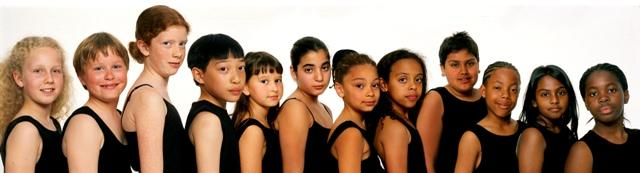
\includegraphics[width=15cm]{figures/colorskin}
\caption{Příklady druhů pigmentace kůže\cite{skincolor:obr}}
\label{colorskin}
\end{figure}

\subsection{Vnější podněty}
Problém pro identifikování chodce v~obraze může také představovat druh osvětlení scény, případně střídání dne a~noci pro venkovní kamerové systémy. Také zde hraje důležitou roli nastavení a~vlastnosti dané kamery. 

\subsection{Oblečení a~různé doplňky}
Do této kategorie spadá například zimní oblečení, které většinou zvětšuje objem či tvar těla, nebo různě rozměrné pokrývky hlavy. Chodec také může nést nějaké předměty, které mohou zakrývat jeho části těla nebo s~ním dokonce splývat. Tyto aspekty také ovlivňují správnost detekce.

\subsection{Pozice v~obraze}
Osoby se mohou nacházet libovolně v~obraze, mohou jít čelem k~ohnisku kamery nebo být zachyceny pouze z~boku. Například kamera umístěná ve výšce pouličního osvětlení v~nějakém předem určeném úhlu snímá obraz z~určité perspektivy. Tato kamera pak zajištuje velikou škálu chodců v~různém měřítku. Pro stroj tohle může být problematické. Osoby ve větším měřítku mohou být snadno detekovatelné, ovšem chodci, kteří jsou hodně vzdálení v~obraze, nikoliv. V~tomto případě také závisí na nastavení daného detektoru za cenu pomalejšího výkonu, získáme přesnější detekci. 

\subsection{Pozadí (prostřední scény)}
Chodci se většinou pohybují v~komplexním venkovním prostředí. Opět, pro lidské oko může být člověk snadno identifikovatelný, a~pro doménu strojů se může tato situace jevit jako neproveditelná. Osoba v~obraze může totiž dokonale splynout s~prostředním, které se za ní nachází.  

Příklad výše zmíněných výzev a~problémů detekce najdeme na obrázku \ref{pedestrians}, který je umístěn níže. Na tomto ilustrativním obrázku najdeme osoby s~různě barevným oblečením různého tvaru. Chodci se zde nacházejí v~různém úhlu k~ohnisku kamery. 

\begin{figure}[H]
\centering
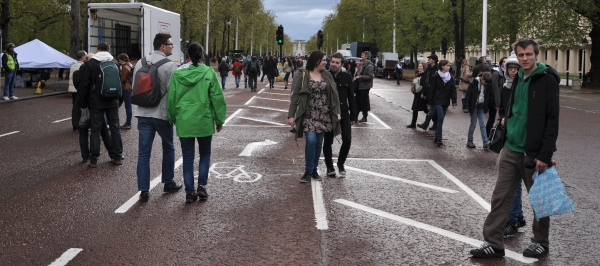
\includegraphics[width=15cm]{figures/pedestrians}
\caption{Ukázka chodců v~obraze}
\label{pedestrians}
\end{figure}
\section{Metody detekce}
V této kapitole budou popsány nejpoužívanější a nejznámější detekční metodiky. Všechny tyto metodiky jsou dostupné minimálně v jedné knihovně, použité v této práci.  

\subsection{Metody založené na příznacích}
Navzdory všem výzvám a problémům detekci chodců, zůstává tato oblast výzkumu stále aktivní a byla navržena řada přístupových technik.
%@TODO
\subsubsection*{Histogram orientovaných gradientů}

Tato metoda vznikla v roce 2005 za účelem detekování chodců v obrazech a je založena na histogramech orientovaných gradientů (\textit{HOG - Histogram of Oriented Gradients}). Autoři této metodiky jsou N. Dalal a B. Triggs \cite{hog:dalal}. Základní myšlenkou je, že místní vzhled a~tvar objektu může být často charakterizován distribucí intenzity gradientů nebo směry hran, aniž by byly přesně známy odpovídající gradientové nebo hranové polohy.  
Prvním krokem před samotným výpočtem příznaků by mělo dojít k zajištění normalizaci barev a gamy, v případě černobílých obrázků normalizaci kontrastu. Tento krok může být ovšem vynechán, jak zdůrazňují autoři Dalal a Triggs. Normalizace deskriptorů dosahují stejného výsledku, a tedy předběžné zpracování obrázku má malý vliv na výkon. Místo toho je prvním krokem výpočet gradientních hodnot. Nejběžnější metodou je aplikování 1-D derivační masky v jednom nebo obou horizontálních a vertikálních směrů. Autoři také experimentovali s komplexnějšími masky, jako je například $3x3$ Sobelova maska nebo diagonální masky, avšak tyto masky se prokázaly jako méně účinné. Stejně tak neúčinné bylo použití jakéhokoliv vyhlazení obrazu před aplikací derivační masky. Tedy nejlepší kombinací parametrů bylo použití konvolucí Gaussovského filtrování $\sigma = 0$ na obraze $I$ s maskou $[-1, 0, 1]$, $[-1,0,1]^\top$:
\begin{equation}
\centering
 \label{eq:hogMask}
 \begin{aligned}
I_x = I * [-1, 0, 1], \\
I_y = I * [-1, 0, 1]^\top
 \end{aligned}
\end{equation}
kde:
\begin{itemize}[label=]
  \item $*$: konvoluce,
  \item $I$: obraz.
\end{itemize}

Druhém kroku dochází k vytvoření histogramu v každé buňce. Každý pixel v buňce má svou váhu, který se podílí na vytvoření orientovaného histogramu, založeného na hodnotách nalezených ve výpočtu gradientu. Samotné buňky jsou rovnoměrně rozloženy do 9 kanálů (binů) po \ang{20}. Pokud buňka vyjde na pomezí úhlu, přičte se její magnituda do obou těchto binů.
Tyto buňky spojíme do větších propojených bloků z důvodu normalizace osvětlení a kontrastu. Pro chodce se používá L2-norm normalizace \ref{eq:normHog}. Tyto bloky se typicky překrývají, což znamená, že každá buňka přispívá více než jednou do finálního deskriptoru. Proces zpracování deskriptoru je ilustrován na obrázku \ref{hog_chain}. Existují dvě varianty spojení bloků, tzv. obdélníkové bloky (R-HOG) a kruhové bloky (C-HOG), viz obrázek \ref{variants_block}.  
\begin{equation}
\centering
 \label{eq:normHog}
 \begin{aligned}
L2-norm&: \qquad  f =& \frac{v}{\sqrt{\lVert v \lVert_2^2 + e^2}} \\
L1-sqrt&: \qquad  f =& \sqrt{\frac{v}{\lVert v \lVert_1 + e}}
 \end{aligned}
\end{equation}
Nechť $v$ je nenormalizovaný vektor obsahující všechny histogramy v daném bloku, $\lVert v \lVert_k$ je jeho k-norm pro $k = 1,2$, a $e$ je malá konstanta.
 \begin{figure}[H]
\centering
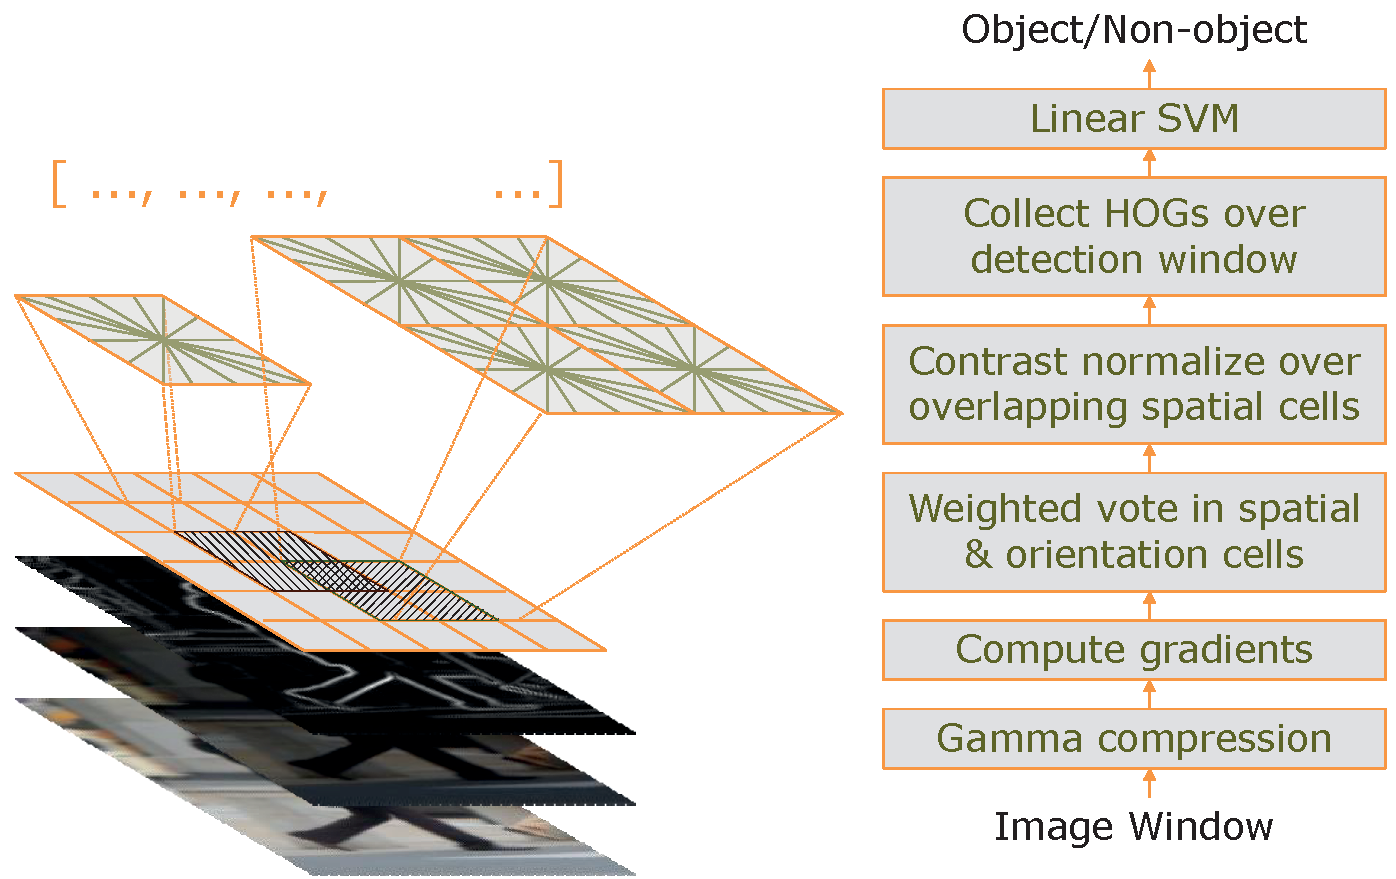
\includegraphics[width=16cm]{figures/hog_pipeline}
\caption{Procesní řetezec výpočtu deskriptoru \cite{hog:dalal}}
\label{hog_chain}
\end{figure}

\textbf{C-HOG} (Kruhové HOG bloky) - lze nalézt ve dvou variantách: \textit{s jedinou, centrální buňkou} a \textit{úhlově rozdělenou centrální buňkou}. Dají se popsat čtyřmi parametry: počtem úhlů a radiálních kanalů (binů), poloměrem centrálního binu a faktorem roztažení pro poloměr dalších radiálních binů.  Tyto bloky se podobají deskriptorům kontextu tvarů (shape context descriptors \cite{shapeContext}), ale C-HOG obsahují buňky s několika orientovanými kanály, zatím co shape context využívají přítomnost jediné hrany.

\textbf{R-HOG} (Obdélníkové HOG bloky) - tyto bloky jsou v praxi nejčastěji používané a reprezentují se třemi parametry: \textit{počet buněk na blok}, \textit{počet pixelů na buňku} a \textit{počet binů (kanálů) na jeden histogram}. Bloky se zdají trochu podobné deskriptorům transformací příznaků invariantní vůči měřítku (scale-invariant feature transform SIFT \cite{siftPaper}). Avšak liší se výpočtem bloků. R-HOG bloky jsou vypočteny v hustých mřížkách v libovolném měřítku bez zarovnání orientace, zatímco SIFT deskriptory obvykle v řídkých, obrazové body invariantní vůči měřítku jsou otočeny, aby přiléhaly orientaci. R-HOG bloky se také používají pro kódování informací. 
\begin{figure}[H]
  \centering
  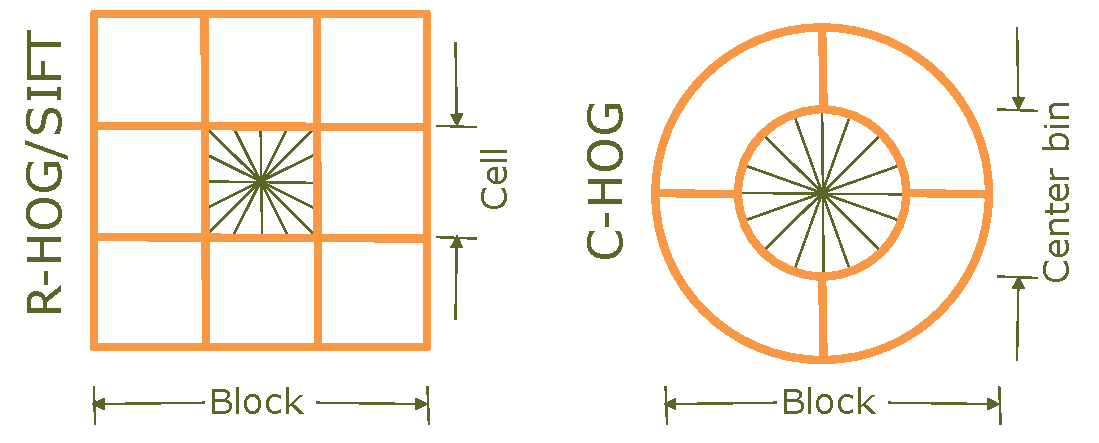
\includegraphics[width=14cm]{figures/hog_variants.pdf}
  \caption{Varianty geometrie spojení bloků \cite{hog:dalal}}
  \label{variants_block}
\end{figure}
V knihovně OpenCV existuje funkce ``detectMultiScale'', která pomocí \textbf{posuvného okénka} (sliding window) projde napříč celým obrazem a v každém tomto okně se vypočítávají vlastnosti. Jeho velikost můžeme definovat pomocí parametru, standardní velikost je $64x120$ a následující popis a výpočty budou odpovídat této velikosti posuvného okna.  

V tomto okně se obrázek rozdělí na $8x8$ bloků a v každém bloku se vypočte histogram a jeho hrany rozdělíme do 9 binů. Vyjde nám vektor o velikosti 9 a tyto vektory spojíme do bloků o velikosti $16x16$ a normalizujeme je na velikost 1, aby byly nezávislé na osvětlení, dostaneme tedy vektor o velikosti 36. Na konci tohoto procesu všechny vektory spojíme a získáme vektor všech příznaků z konkrétního vzorku nebo z oblasti zájmu posuvného okénka. Obrázek \ref{fig:hogCalc} zobrazuje vstup vzorku pro vypočítání jeho příznaků neboli orientovaných hran, kde nejprve obrázek převedeme do černobílé barvy, provedeme normalizaci kontrastu a gamy a následně vypočítáme jeho vektor příznaků.

Tato metodika se běžně používá s lineárním SVM klasifikátorem, a tak je velmi účinná pro jakoukoliv detekci. 
Ukázka dělení obrazového okna je na obrázku \ref{hog_cells}.

 \begin{figure}[H]
\centering
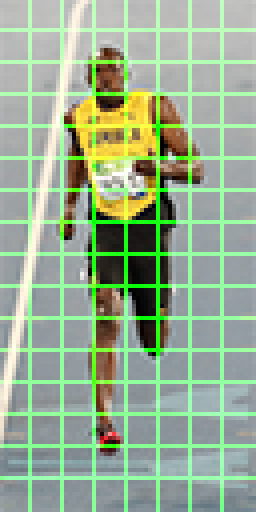
\includegraphics[width=3.6cm]{figures/hog_cells}
\caption{Rozdělení obrazu do $8\times8$ buněk. \cite{hog:obr}}
\label{hog_cells}
\end{figure}

\begin{figure}[H]
\centering
\begin{minipage}{.3\textwidth}
  \centering
  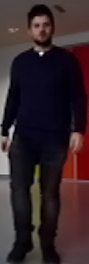
\includegraphics[width=.5\linewidth]{figures/hog_input}
  \caption*{Vstupní obrázek}
  \label{fig:hog_input}
\end{minipage}%
\begin{minipage}{.3\textwidth}
  \centering
  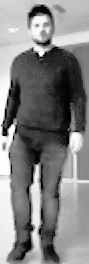
\includegraphics[width=.5\linewidth]{figures/hog_histogram_before}
  \caption*{Normalizace kontrastu}
  \label{fig:hog_contrast}
\end{minipage}%
\begin{minipage}{.3\textwidth}
  \centering
  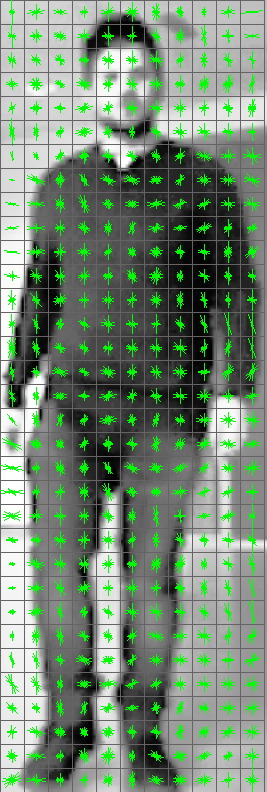
\includegraphics[width=.5\linewidth]{figures/features}
  \caption*{Výpočet příznaků}
  \label{fig:hog_features}
\end{minipage}
\caption{Normalizace a výpočet příznaků pro obrázek}
\label{fig:hogCalc}
\end{figure}

\subsubsection*{Haarovy příznaky} % #TODO
Na tomto přístupu je založen objektový detektor Viola-Jones \textit{Viola-Jones object detector framework}, který poskytuje v reálném čase spolehlivou a konkurenceschopnou detekci objektů. Tento systém byl navržen v roce 2001 a i když může být vycvičen pro detekci různých objektových tříd, byl primárně použit především pro detekci obličeje. Detektor pracuje s obrazy ve stupně šedi a skládá se ze tří částí. Z integrálního obrazu, Haarových příznaků a AdaBoost algoritmu. 

Integrální obraz je takový obraz (obrázek \ref{fig:integralimage}), kde každý bod $x$ představuje součet hodnot předchozích pixelů doleva a nahoru. Spodní pravý bod obsahuje součet všech pixelů v obraze.
Zápis integrálního obrazu je
\begin{equation*}
\label{integralimage}
 I(x, y) = \sum_{\substack{x' \leq x \\ y' \leq y}}{} i(x', y'),
\end{equation*}
kde $i(x', y')$ je hodnota pixelu na pozici $(x, y)$.
\begin{figure}[H]
\centering
\begin{minipage}{.4\textwidth}
  \centering
  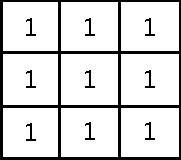
\includegraphics[width=.5\linewidth]{figures/ii_input}
  \caption*{Vstupní obraz}
  \label{fig:ii_input}
\end{minipage}%
\begin{minipage}{.4\textwidth}
  \centering
  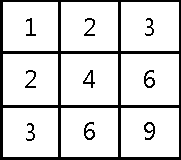
\includegraphics[width=.5\linewidth]{figures/ii_output}
  \caption*{Integrální obraz}
  \label{fig:ii_output}
\end{minipage}
\caption{Převod obrazu na integrální obraz}
\label{fig:integralimage}
\end{figure}

Všechna lidská těla a obličeje sdílejí některé podobné rysy a ty mohou být porovnány pomocí Haarových příznaků.
\begin{itemize}
  \item{Oční oblast je než tmavší než oblast nosního mostu.}
  \item{Proporce lidského těla.}
  \item{Hlava člověka je tmavší než její okolí.}
  \item{Oblast mezi dolními končetinami je světlejší než samotné nohy.}
\end{itemize}
Sada Haarových vlnek je na obrázku \ref{fig:basichaarfeatures}, jedná se pouze o základní sadu příznaků.
\begin{figure}[H]
\centering
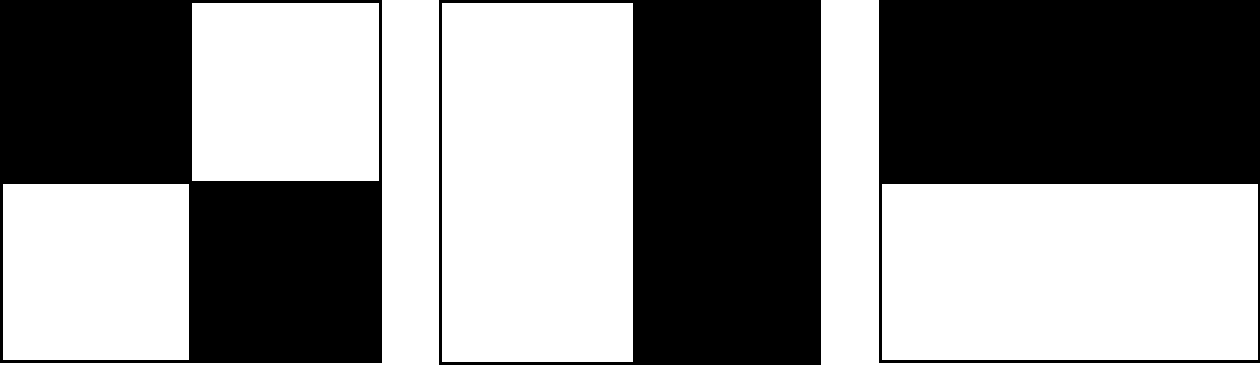
\includegraphics[width=.7\linewidth]{figures/haar_features}
\caption{Základní sada Haarových příznaků}
\label{fig:basichaarfeatures}
\end{figure}

Pro identifikaci lidských postav se používá rozšířená sada vlnek, tzv. Haar-like příznaky. V některých vědeckých publikacích byly představy prototypy těchto příznaků. Na obrázku \ref{fig:haarlike} jsou některé z nich. Hodnota příznaku je rozdíl mezi sumou pixelů pod bílou a černou oblastí Haarových vlnek.
\begin{figure}[H]
\centering

\includegraphics[width=.6\linewidth]{figures/haar_like}
\caption{Vybrané prototypy Haar-like příznaků}
\label{fig:haarlike}
\end{figure}

\subsubsection*{Lokální binární vzor} %&TODO
Metoda LBP (Local Binary Pattern) byla navržena pro klasifikaci textur v obrazech v roce 1990. \cite{lbp:texture} Poprvé však byly popsány až v roce 1994. \cite{lbp:first} Hlavní myšlenkou LBP, že struktury obrazu mohou být efektivně zakódovány porovnání všech pixelů se sousedními pixely. Výsledkem

Prvním krokem této metody je převod obrazu do stupně šedi a jeho rozdělení do buněk. Okolní hodnoty pixelů jsou porovnávány se středovým pixelem, pokud je jejich hodnota rovna nebo větší zapíše se na tuto pozici jednička v opačném případě nula. Tyto hodnoty seřadíme buď podle hodinových ručiček nebo naopak a získáme 8-místné binární číslo, které převedeme do dekadické soustavy. Následujícím kroku z čísel, které jsme získali kombinací pixelů v buňkách vypočítáme histogram. V posledním kroku zřetězíme všechny histogramy buněk a získáme vektor příznaků pro celý obraz. Jedná se o 256-dimenzionální vektor příznaků. 
Matematicky lze LPB vyjádřit jako
\begin{equation*}
LBP_{P,R} = \sum_{p=0}{P-1} s(g_p - g_c)2^P, \\
s(x) =
  \begin{cases} 
   1 & \text{pro } x \geq 0 \\
   0       & \text{pro } x < 0
  \end{cases}
\end{equation*}
kde: $P$ je počet bodů v okolí, $R$ vyjadřuje vzdálenost bodů od středového pixelu, $g_c$ je středový pixel $g_p$ je aktuální pixel. 

Následující příklad se vztahuje k obrázku \ref{fig:lbpsum}. Po porovnání pixelů se středovým pixelem, jsme získali vzor $11110001$. Tento vzor převedeme do dekadické soustavy a sečteme, $ 1+16+32+64+128 = \textbf{241}$. Získali jsme hodnotu této buňky do vektoru příznaků.

\begin{figure}[H]
\centering
\begin{minipage}[b]{.3\textwidth}
  \centering
  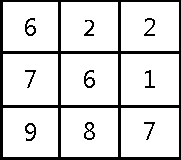
\includegraphics[width=.5\linewidth]{figures/lbp_img}
  \caption*{Vstupní buňka}
  \label{fig:lpbimg}
\end{minipage}%
\begin{minipage}[b]{.3\textwidth}
  \centering
  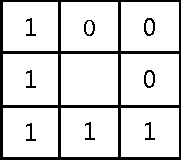
\includegraphics[width=.5\linewidth]{figures/lbp_thresh}
  \caption*{Prahové hodnoty}
  \label{fig:lbpthresh}
\end{minipage}
\begin{minipage}[b]{.3\textwidth}
  \centering
  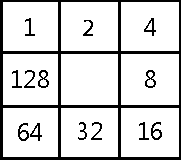
\includegraphics[width=.5\linewidth]{figures/lbp_weights}
  \caption*{Váhově ohodnoceny pixely}
  \label{fig:lbpweights}
\end{minipage}
\caption{Výpočet příznaku}
\label{fig:lbpsum}
\end{figure}

Výhoda této metody je její rychlý a snadný výpočet a odolnost vůči různým osvětlením. Na druhou stranu je těžší na trénování, protože výsledné dekadické číslo může mít obrovské množství možností (podle parametru $P$). K omezení můžeme využít uniformní vzory (viz obrázek \ref{fig:lbpvzory}), které vyfiltrují možné okolí. Pro parametr $P=8$, získáme 59 vzorů. 

\begin{figure}[H]
\centering
\begin{minipage}[b]{.18\textwidth}
  \centering
  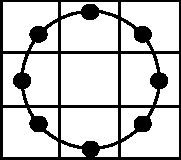
\includegraphics[width=.9\linewidth]{figures/lbp_spot}
  \caption*{Spot}
\end{minipage}
\begin{minipage}[b]{.18\textwidth}
  \centering
  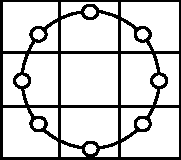
\includegraphics[width=.9\linewidth]{figures/lbp_spot_flat}
  \caption*{Spot/Flat}
\end{minipage}
\begin{minipage}[b]{.18\textwidth}
  \centering
  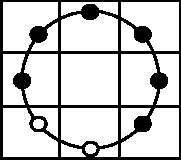
\includegraphics[width=.9\linewidth]{figures/lbp_line}
  \caption*{Line}
\end{minipage}
\begin{minipage}[b]{.18\textwidth}
  \centering
  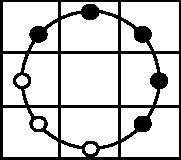
\includegraphics[width=.9\linewidth]{figures/lbp_corner}
  \caption*{Corner}
\end{minipage}
\begin{minipage}[b]{.18\textwidth}
  \centering
  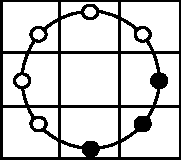
\includegraphics[width=.9\linewidth]{figures/lbp_edge}
  \caption*{Edge}
\end{minipage}
\caption{Lokální okolí LBP metody}
\label{fig:lbpvzory}
\end{figure}

Pro detekování chodců v obrazech se LPB kombinují s metodou HOG. \cite{hoglpb}

\subsubsection*{HOG + LBP}
\subsubsection*{HOG + SVM ? }

\subsection{Další metody v kombinaci se segmentací nebo detekci pohybu} % @TODO 

\subsection{Klasifikátory}
\subsubsection*{SVM} % @TODO
Support vector machines (SVM) jsou učební modely, které jsou velmi populární v oblasti strojového učení. Původně tato technika sloužila k vytvoření optimálního binárního klasifikátoru, později byla rozšířena do regresního a clustering problémů. Tato metoda je založena na tzv. jádrových algoritmech (kernel machines) s využitím podpůrných vektorů (support vectors).

Primárním cílem SVM je nalézt nadrovinu, která optimálně rozděluje prostor příznaků tak, aby trénovací data náležela do konkrétních tříd, viz obrázek \ref{fig:svm}. Pokud mezera mezi oddělující nadrovinou a nejbližšími vektory příznaků z obou kategorií (v případě binárního klasifikátoru) je maximální, jedná se o optimální řešení. Vektory příznaků v blízkosti této nadroviny se nazývají podpůrné vektory, což znamená, že pozice ostatních vektorů nemá vliv na nadrovinu (rozhodovací funkce). 

Jinými slovy, se jedná o diskriminační klasifikátor formálně definovaný rozdělovací nadrovinou, která kategorizuje nové příklady.
\begin{figure}[H]
\centering
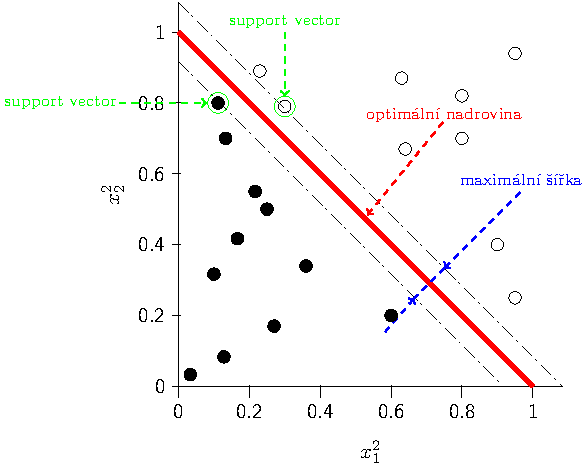
\includegraphics[width=.7\linewidth]{figures/svm.pdf}
\caption{Optimální oddělovací hranice}
\label{fig:svm}
\end{figure}

Implementaci SVM můžeme nalézt již v existujících knihovnách jako jsou například LIBSVM, MATLAB, SAS, SVMLight a další. V následující části bude popsána knihovna LIBSVM, na které je založena implementace v OpenCV a v Dlibu.  

Tato knihovna byla napsána v roce 2001 \cite{libsvm} a stále se vyvíjí. Podporuje různé formulace SVM pro odhady klasifikace, regrese a distribuce.

\paragraph*{$C$-Support vektorová klasifikace (C-SVC)}
Umožnuje nedokonalé oddělení tříd pro n-tříd ($n > 2$) s postihovým multiplikátorem $C$, pro odlehlé hodnoty ($C > 0$). \cite{csvmclass}

\paragraph*{$\nu$-Support vektorová klasifikace ($\nu$-SVC)}
$n$- třídní klasifikace s možností nedokonalé separace. Tato klasifikace přidává nový parametr $\nu \varepsilon (0,1]$ a čím větší je jeho hodnota tím hladší je rozhodovací funkce. \cite{nusvmsvrclass}

\paragraph*{Distribuční odhad (Jednotřídní SVM)}
Distribution Estimation (One-class SVM), jak název, již sám o sobě napovídá, všechny tréninková data pocházejí z jedné třídy, SVM vytvoří hranici, která odděluje třídu od zbývající části. \cite{oneclasssvm}

\paragraph*{$\varepsilon$-Support vektorová regrese ($\varepsilon$-SVR)}
Vzdálenost mezi vektory příznaků a rozdělovací nadrovinou musí být menší než $p (\varepsilon)$. Pro odlehlé hodnoty opět použijeme multiplikátor $C$. Musí tedy platit: $C > 0$ a $\varepsilon > 0$. \cite{svrsvm}

\paragraph*{$\nu$-Support vektorová regrese ($\nu$-SVR)}
Tato klasifikace je podobná jako $\varepsilon$-SVR. Na místo p se použije parametr $\nu \varepsilon (0,1]$. \cite{nusvmsvrclass}

Účinnost SVM závisí na výběru správného jádra a parametry jádra. Nejběžněji se používá Gaussovo jádro s jedním parametrem $\gamma$. V této knihovně se můžeme setkat s následujícími jádry.

\paragraph*{Lineární jádro}
Použití tohoto jádra je velmi rychlé (bez jakékoliv transformace), jedná se lineární diskriminaci a rozdělovací nadrovina bude vždy přímka. Pro toto jádro platí 
\begin{equation*}
 \label{linearK}
  K(x_i, x_j) = x_i^T x_j,
\end{equation*}
  kde $x_i$ a $x_j$ jsou vektory vstupního prostoru.

\paragraph*{Polynomické jádro}
Polynomické jádro umožňuje učení nelineárních modelů
\begin{equation*}
\label{polyK}
  K(x_i, x_j) = (\gamma x_i^T x_j + c)^{d}, \gamma > 0,
\end{equation*}
kde: $c \geq 0$, volný parametr, který vylučuje vliv vyššího řádu oproti polynomu nižšího řádu (pokud $c = 0$, jádro je homogenní), řád polynomu určuje parametr $d$.

\paragraph*{Gaussovo jádro}
Gaussovo neboli RBF (Radial Basis Function) jádro se řadí mezi nejpoužívanější a je definované jako
\begin{equation*}
\label{RBFK}
 K(x_i, x_j) = e^{-\gamma ||x_i - x_j||^2}, \gamma > 0,
\end{equation*}
kde: $||x_i - x_j||^2$ značí kvadratickou euklidovskou vzdálenost mezi dvěma vektory příznaků.

\paragraph*{Sigmoidní jádro}
toto jádro je podobné sigmoidní funkci v logistické regresi
\begin{equation*}
\label{sigmK}
 K(x_i, x_j) = \tanh(\gamma x_i^T x_j + r),
\end{equation*}
kde $r$ je volitelný parametr.

\paragraph*{Exponenciální jádro}
Exponenciální jádro $\chi$2 je podobné RBF jádru a využívá se převážně na histogramy
\begin{equation*}
\label{expK}
 K(x_i, x_j) = e^{-\gamma \chi^2(x_i,x_j)}, \chi^2(x_i,x_j) = \frac{(x_i-x_j)^2}{(x_i+x_j)}, \gamma > 0,
\end{equation*}

\paragraph*{Jádro histogramu průsečíků}
Toto jádro je také známé jako \textit{Min Kernel}, jedná se o nejnovější jádro v této knihovně a je velmi rychlé a užitečné při klasifikaci
\begin{equation*}
\label{innK}
 K(x_i, x_j) = min(x_i,x_j).
\end{equation*}

Nejpoužívanější jádra jsou ilustrována v následujícím obrázku \ref{kernels}.
\begin{figure}[ht] 
  \begin{minipage}[b]{0.5\linewidth}
    \centering
    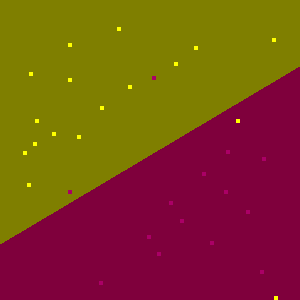
\includegraphics[width=.6\linewidth]{figures/linear} 
    \caption*{Lineární jádro} 
    \vspace{4ex}
    \label{linearKernel} 
  \end{minipage}%%
  \begin{minipage}[b]{0.5\linewidth}
    \centering
    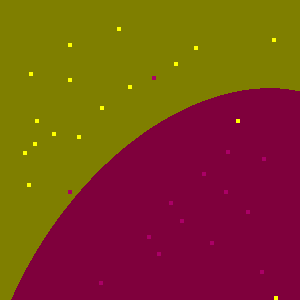
\includegraphics[width=.6\linewidth]{figures/poly} 
    \caption*{Polynomické jádro} 
    \vspace{4ex}
    \label{polyKernel} 
  \end{minipage} 
  \begin{minipage}[b]{0.5\linewidth}
    \centering
    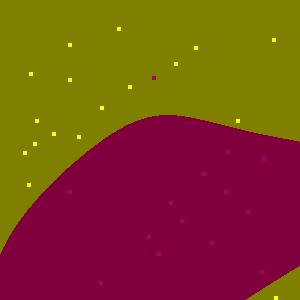
\includegraphics[width=.6\linewidth]{figures/rbf} 
    \caption*{Gaussovo jádro} 
    \vspace{4ex}
    \label{rbfKernel} 
  \end{minipage}%% 
  \begin{minipage}[b]{0.5\linewidth}
    \centering
    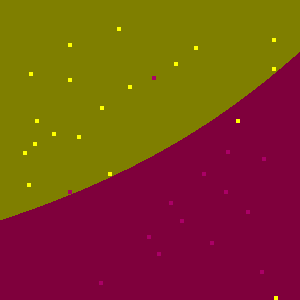
\includegraphics[width=.6\linewidth]{figures/sigm}
    \caption*{Sigmoidní jádro} 
    \vspace{4ex}
    \label{sigmKernel} 
  \end{minipage} 
  \caption{Ilustrační obrázek jader při použití $C$-SVM \cite{libsvm}}
  \label{kernels} 
\end{figure}

SVM je výsledek práce několika lidí po mnoho let. Prvním algoritmem této problematiky je přisuzovaný Vladimíru Vapnikovi v roce 1963 \cite{svm:vapnik}. V reálném životě byly úspěšně použity ve třech hlavních oblastech: kategorizace textu, rozpoznání obrazu a bioinformatika. Mezi konkrétní příklady patří třídění novinových zpráv, rozpoznávání ručně psaných čísel nebo například vzorky rakovinových tkání.

\subsubsection*{Kaskádové klasifikátory} % @TODO
Kaskádový klasifikátor se skládá z více slabších klasifikátorů umístěné v kaskádách za sebou. Požadavky na tento druh klasifikátoru byla rychlost detekce, aby mohl být implementován na procesorech s nižším výkonem, například v kamerách nebo v telefonech. Princip tohoto klasifikátoru je velice jednoduchý a prostý. Klasifikátor na první vrstvě může vyfiltrovat většinu negativních oken. Na druhé vrstvě se mohou odfiltrovat ``těžší'' negativní okna, která přežila z první vrstvy a tak dále. Sub okno, které přežije všechny tyto vrstvy bude označeno jako pozitivní detekce. Příklad řetězce kaskádového klasifikátoru je ilustrován v obrázku \ref{fig:ccpipeline}, kde $K1$-$KN$ je klasifikátor první až n-té vrstvy.

Klasifikátory si mezi sebou předávají všechny informace o vstupním obraze. Tímto kaskádovým vyhodnocováním se může redukovat čas, nutný pro detekci v daném obraze. Prvním takovým klasifikátorem byl detektor obličeje Viola-Jones \cite{violajones}.  
\begin{figure}[H]
\centering
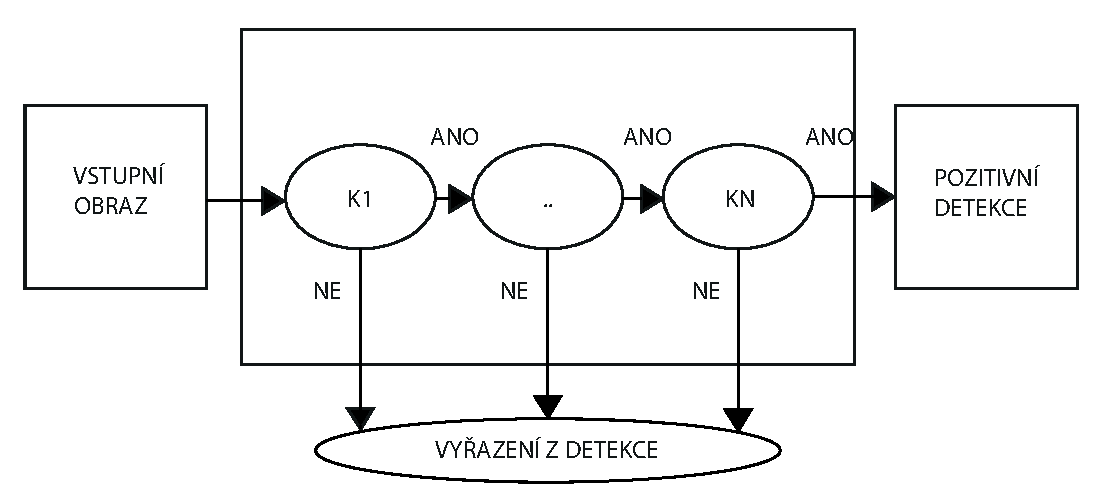
\includegraphics[width=.7\linewidth]{figures/cascadeClass.pdf}
\caption{Ukázka pipeline kaskádového klasifikátoru}
\label{fig:ccpipeline}
\end{figure}

\subsubsection*{AdaBoost}
\textbf{AdaBoost}, neboli Adaptive Boosting byl představen v práci pánů Freund a Schapire \cite{adaboost}. Tento klasifikátor kombinuje slabé klasifikátory k vytvoření jednoho silného klasifikátoru. V kombinaci více klasifikátorů s výběrem trénovací sady v každé iteraci algoritmu a přidělení správné váhy na konci trénování, docílíme klasifikátoru s dobrou přesností. Klasifikátory v tomto řetězci, které mají klasifikační přesnost menší než 50\% jsou ohodnoceny zápornou vahou. Váhou nula jsou ohodnoceny klasifikátory, které mají přesnost 50\%. Pouze ty, co mají přesnost vyšší než 50\% jsou přínosné do této kombinace a můžeme hovořit o zesílení (boosting) klasifikace. 

\subsection{Deep learning}
\section{Dataset} % @TODO 
\section{Použité knihovny}
Na internetu je spousta dostupných či placených knihoven pro zpracování obrazu. Avšak nejznámější a~nejpoužívanější knihovnou pro zpracování obrazu je OpenCV \cite{opencvdoc}. Tato knihovna je dostupná na většinu platforem a~z~tohoto důvodu jsem jí v~práci použil. Dále jsem v~práci použil knihovnu Dlib \cite{dlibdoc}, která je taky volně dostupná na internetu a~také se jedná o multiplatformní knihovnu. Obě tyto knihovny budou popsány v~následujících dvou podsekcí.
\subsection{Knihovna OpenCV}
OpenCV (\textit{Open Source Computer Vision Library}) je open-source knihovna, která slouží k~zpracování obrazu a~k~strojovému učení. Je psaná v~C/C++ jazyce s~podporou multijádrového zpracování.

Knihovna má více než 2500 optimalizovaných algoritmů, které zahrnují obsáhlé sady klasických a~moderních algoritmů pro zpracování obrazu a~strojové učení. Tyto algoritmy mohou být použity na detekci a~rozpoznávání tváří, identifikování objektů, vyhodnocování lidských akcí ve videosekvencích, sledování pohybů pomocí kamery, sledování pohybujících se objektů, extrahování 3D modelů z~objektů, vytváření 3D mračen bodů ze stereo kamer, spojování obrazu do jednoho s~vysokým rozlišením na dané scéně, hledání podobných obrazů z~obrazové databáze, odstranění červených očí z~obrazu způsobené bleskem, sledování pohybu očí, rozeznání scenérie a~vytvoření značek pro překrytí rozšířenou realitou a~další.

Knihovna má rozhraní pro jazyky C++, C, Python, Java a~MATLAB a~podporuje operační systémy Windows, Linux, Android, iOS a~MacOS. 
Pokud jsou dostupné MMX a~SSE instrukce tak knihovna je použije pro zvýšení jejího výkonu.

Podílí se na ní komunita lidí, kterou tvoří více než 47 tisíc uživatelů celého světa a~přesahuje více než 14 milionů stažení. 

%OpenCV leans mostly towards real-time vision applications and takes advantage of MMX and SSE instructions when available. A full-featured CUDA and OpenCL interfaces are being actively developed right now. There are over 500 algorithms and about 10 times as many functions that compose or support those algorithms. OpenCV is written natively in C++ and has a templated interface that works seamlessly with STL containers. 
%OpenCV (Open Source Computer Vision Library) is released under a BSD license and hence it’s free for both academic and commercial use. It has C++, C, Python and Java interfaces and supports Windows, Linux, Mac OS, iOS and Android. OpenCV was designed for computational efficiency and with a strong focus on real-time applications. Written in optimized C/C++, the library can take advantage of multi-core processing. Enabled with OpenCL, it can take advantage of the hardware acceleration of the underlying heterogeneous compute platform.

%Adopted all around the world, OpenCV has more than 47 thousand people of user community and estimated number of downloads exceeding 14 million. Usage ranges from interactive art, to mines inspection, stitching maps on the web or through advanced robotics.

Z~této knihovny byly použité následující nástroje:

\begin{itemize}
  \item{Mixtura Gausiánů,}
  \item{Konvexní obal,}
  \item{Histogram orientovaných gradientů,}
  \item{Support vector machines.}
\end{itemize}
\subsection{Knihovna Dlib}
Autorem této knihovny je Davis King. Jedná se o~moderní C++ knihovnu obsahující algoritmy pro strojové učení a~nástroje pro vytváření komplexních programů v~jazyce C++. Používá se jak v~industriální, tak v~akademické sféře v~široké škále oblastí, jako jsou zejména vestavěná zařízení, robotika, mobilní telefony a~velkých, výkonných výpočetních prostředí. Jedná se o~sbírku nezávislých softwarových komponent, kde každá z~nich je doprovázena důkladnou dokumentací a~mnoha příklady použití.

Jádrem filozofie této knihovny je věnování se snadnému používání a~přenositelnosti. Proto je kód navržen tak, aby nebylo po uživateli vyžadováno cokoli ručně konfigurovat nebo instalovat. K~dosažení tohoto cíle je veškerý kód specifický a~pro konkrétní platformu omezen a~obalen pomocí API rozhraní. Všechno ostatní je buď navrstveno na těchto obalech nebo napsané v~normě ISO standardu C++. 

Knihovna se stále rozrůstá hlavně díky dobrovolným přispěvovatelům a~v~době psaní práce obsahuje například i~softwarové komponenty pro práci se sítí, vlákna, grafické rozhraní, komplexní datové struktury, lineární algebru, statistické strojové učení, zpracování obrazu, data mining, XML a~parsování textu, numerickou optimalizaci, Bayeské sítě. V~uplynulých letech byla velká část vývoje zaměřena na širokou sadu nástrojů statického strojového učení, avšak knihovna zůstává univerzální.  

V~současné době je známo, že knihovna pracuje na systémech OS X, MS Windows, Linux, Solaris, BSD, HP-UX. Knihovna by měla také pracovat na libovolné platformě POSIX, ale není otestovaná na všech dostupných verzích. 
Z~této knihovny byl v~práci použit pouze FHOG detektor objektů.
%Knihovna Dlib je vyvíjena primárně Davidem Kingem, který je jejím autorem a její počátky tkví již v roce 2002. Tato knihovna je otevřená, multiplatformní a navržena designově na zakázku a komponenty jsou založeny na softwarovém inženýrství, jedná se o sbírku nezávislých softwarových komponent z nichž je každá doprovázena důkladnou dokumentaci a mnoha příklady použítí.


 
\section{Aplikace}
Aplikace je napsaná v~nativní C++--11, ve vývojovém prostředí Visual Studio 2015. Jedná se o~multiplatformní konzolovou aplikaci, která byla primárně určena pro systémy ARM s~operačním systémem Linux. 

Její obsluha je jednoduchá a~funguje na bázi argumentů, které určují její chování. Nastavení parametrů se provádí přes externí soubor, což umožňuje jednodušší a~pohodlnější manipulaci s~aplikací. Disponuje širokým spektrem nástrojů od testování klasifikátorů, po jejich trénování až po samotnou detekci. Její nástroje jsou popsány v~následujících podsekcích.

\subsection{Detekování chodců}
Hlavním účelem této aplikace je detekování chodců v~obrazech. Aplikace umožnuje detekování chodců ve videosekvencích, obrázcích a~také z~webové kamery. Díky externímu nastavení práhů detektorů a~jiných proměnných lze měnit nastavení bez opětovného kompilování aplikace. Díky anotovácímu nástroji, který je součástí aplikace, lze oblasti chodců zaznamenat do souboru, kterým se vyhodnotí výstup detektoru.
 
Obrázek \ref{mog_algorithm} ilustruje průběh algoritmu při volbě detekce pomocí metody MOG a~HOG. Prvním krokem algoritmu je získání snímku z~aktuální videosekvence nebo kamery, pokud obrázek je prázdný, cyklus zde končí. Snímek se následně předzpracovává převodem do stupně šedi a~aplikací rozostřovacího filtru. Tento obrázek je následně zpracováván metodikou substrakce pozadí a~na tento obraz se aplikuje eroze a~dilatace, to proto, aby se v~snímku vyfiltrovaly malé, nevýznamné oblasti a~následně spojily ty větší potencionální, kde se může nacházet chodec. Tyto oblasti se obalí pomocí kontur a~převedou na rámce, díky kterým se z obrazu vystřihnou tyto části. Na získaných oblastech v~následujícím kroku probíhá samotná detekce. Detekční metoda vrátí rámce potencionálních oblastí chodců a~vykreslí se do původního obrazu. Proces se opakuje do té doby, dokud získaný obrázek z~kamery není prázdný. Pokud obrázek po aplikování masky substrakce pozadí neobsahuje dostatečně velké oblasti k~aplikaci rámců, program pokračuje načítáním dalšího obrazce z~kamery.  

\begin{figure}[H]
\centering
\includegraphics[width=14cm]{figures/alg_moghog}
\caption{Algoritmus aplikace při selekci kombinace MoG a~HoG detekce}
\label{mog_algorithm}
\end{figure}

\subsection{Cross validace klasifikátoru}
Cross validace klasifikátoru vůči nějaké sadě negativních a~pozitivních vzorků je nedílnou součástí vytvoření ideálního a~úspěšného klasifikátoru.  Aplikace nabízí cross-validaci OpenCV a~Dlib klasifikátoru. Diskriminační klasifikátor SVM z~OpenCV lze validovat třemi způsoby. První je náhodný přístup, generování trénovacích parametrů klasifikátoru s~různou iterací.

Další efektivnějším způsobem je pomocí diferenciální evoluce. Tento algoritmus vychází z~genetického žíhání. Algoritmus nastaví určitý počet dimenzí pro validaci parametrů SVM a~následně probíhá ``žíhání'' parametrů takřka k~jejich dokonalosti. Tento proces trvá 1000 cyklů.

Posledním druhem validace pro klasifikátor SVM z~OpenCV je obdobný z~Dlib knihovny, jedná se o~vnořené cykly, kde se hrubou silou postupně testují parametry a~výsledek validace se vypisuje do konzole. 

Pro klasifikátor z~Dlib knihovny je použita pouze metodika pro postupné testování parametrů hrubou silou v~cyklech. Výhodou je rozdělení trénovacích dat do 3 množin, kde dvě slouží na trénování a~jedna pro testování a~následně naopak. Tato validace má nejdelší výpočetní čas a~výsledkem je přesnost klasifikátoru pro pozitivní a~negativní množinu vzorků.

\subsection{Testování klasifikátoru}
Testování klasifikátoru je proces, při kterém se otestuje na daných vzorcích, u~kterých známe jejich štítek. Díky této metodice zjistíme, jak spolehlivě je natrénovaná SVM a~jaká je její přesnost detekce. Přesněji řečeno k~daným vzorkům máme soubor Ground truth hodnot, proti kterým se porovnává výstup predikce daného klasifikátoru. 

\subsection{Trénování klasifikátoru}
Program také umožňuje natrénování vlastního klasifikátoru. Parametry se vyberou z~externího souboru s~nastavením. V~tomto souboru jsou také uloženy cesty k~souborům se vzorky. 

Trénovací režim aplikace lze spustit přes argument '-t=train" a~následně je uživateli nabídnut typ trénování. Program zvládne vytrénovat klasifikátor jak z~knihovny OpenCV, tak i~z~knihovny Dlib. 

Trénování klasifikátorů z~OpenCV probíhá naplněním vzorků do paměti včetně jejich kategorizace. Následně pro každý vzorek jsou vypočítané jeho příznaky a~opět uložené do paměti programu. Posledním krokem před trénováním je jejich převod do jednořádkové matice a~poté je spuštěno samotné trénování klasifikátorů. Tento krok trvá v~závislosti na velikosti trénovací matice a~zvolených parametrů. Uživatel může zvolit i~dvojité trénování, za tímto stojí stejný postup, ale na konci trénování se spustí detekce pomocí posuvného okénka na negativních vzorcích a~tyto vzorky budou rozšířeny o~výstup z~detektoru. Tento proces se nazývá Bootstraping. Výstupem trénování je soubor YAML, který je čitelný a~slouží pro serializaci strukturovaných dat. Nalezneme zde parametry, použité pro trénování, vytrénované vzorky a~vektor, který určuje rozdělující přímku.

Další možností je vytrénovaní klasifikátoru z~knihovny Dlib. Trénování je obdobné jako u~předchozí metody. Data jsou načtena jako mapy obrázků a~tyto obrázky se parsují pomocí XML souboru. Trénování probíhá pouze z~pozitivních vzorků. Výstupem je binární soubor s~příponou svm.

Poslední možností trénování je kombinace výše zmíněných postupů. Vzorky se zpracují za pomocí OpenCV knihovny a~vstupem do trénovací metody klasifikátoru z~Dlibu je trénovací matice. Tu je nejprve nutné převést na formát této knihovny a~poté je možné provést trénování.

Podstatný rozdíl mezi těmito binárními klasifikátory je v~rozdílu jejich štítků. OpenCV klasifikátor můžeme definovat štítky libovolně, nejčastější však 1 pro pozitivní vzorky a~0 pro negativní. Zatím co Dlib klasifikátor přijímá pouze 1 pro pozitivní a~zápornou 1 pro negativní vzorky.

Trénování klasifikátoru je velmi náročnou  operací na hardwarové prostředky. Ovšem závisí na trénovací sadě. Sada o~počtu 200 tisíc vzorků zkonzumuje až 16 GB paměti.

\subsection{Anotace chodců v~obraze}
Aplikace také disponuje nástrojem pro anotaci chodců v~obraze. Najednou umožňuje anotovat až 5 chodců a~tyto anotace, i~když to není až tak potřebné pro správnost anotace, jsou od sebe barevně odlišeny. Manipulace s~tímto nástrojem je velmi snadná a~jeho náhled je na obrázku \ref{tool_anotate}.

Klávesami `0' až `4' se přepíná mezi anotacemi, přičemž se tato selekce vypíše pro kontrolu do konzole. Klávesa `r' slouží pro vynulování vybrané anotace. Klávesou `n' přeskočíme aktuální snímek bez uložení anotovaných pozic. Klávesa `s' uloží aktuální anotované pozice do paměti a~přepne se na další snímek, přičemž pozice první anotace zůstane nezměněná, to umožňuje jednodušší práci, pokud se v~obraze nachází pouze jeden chodec. Klávesy `i', `j', `k' a~`l' umožňuje pohyb v~obraze, pro přesnější umístění anotované části. Pokud tyto klávesy stiskneme společně s~klávesou `shift', umožní nám to měnit velikost dané anotace. Klávesa `x' uloží aktuální pozice anotací v~paměti do souboru. Tato funkcionalita umožňuje přerušovanou práci na anotacích videosekvence, ale vyžaduje manuální úpravu souboru uživatelem. Anotovaná část se může překrývat s~jinou. Konkrétní anotace je zobrazena pro kontrolu samostatně zobrazena v~dalším okně.

Všechny tyto oblasti zájmu a~snímek s~anotacemi jsou uloženy na disk v~podobě obrázku pro pozdější kontrolu nebo oblasti zájmu mohou být použity pro trénování nebo cross validaci klasifikátoru. Výstup tohoto nástroje je plně kompatibilní s~evaluační funkcí programu a~jedná se tedy o~Ground truth soubor všech anotací ve videosnímku.
 \begin{figure}[H]
\centering
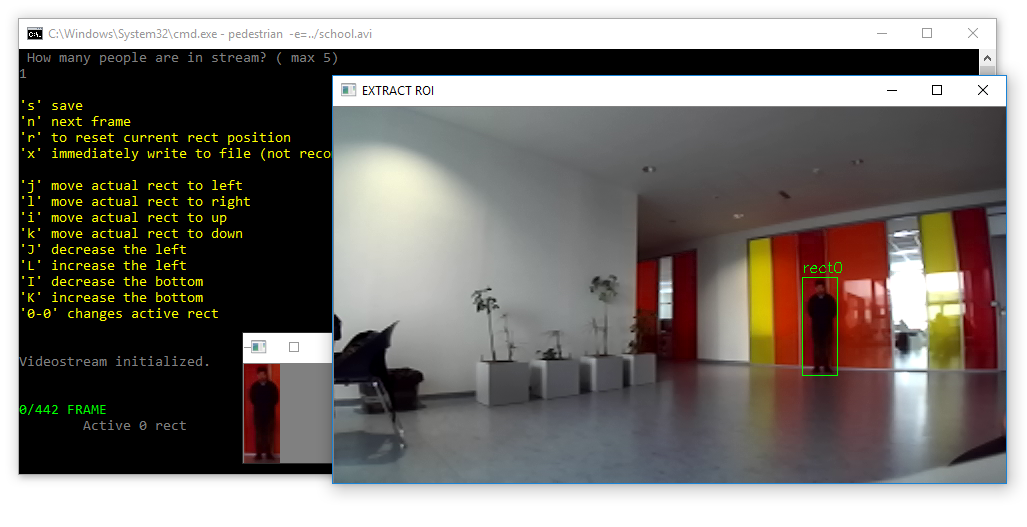
\includegraphics[width=13.5cm]{figures/annotation_example}
\caption{Nástroj pro anotování oblastí chodců}
\label{tool_anotate}
\end{figure}

\subsection{Tvorba negativních vzorků z~obrazu}
Tento nástroj umožňuje vytvořit negativní vzorky pro trénování procházením obrázku pomocí posuvného okénka. Velikost posuvného okénka je definována v~externím souboru. Vstupem je textový soubor s~cestami k~obrázkům.

\section{ARM zařízení}
% @TODO 
\subsection{Použitá zařízení}
K otestování mého programu jsem využil počítače architektury ARM. Jedná se o počítače SolidRun HummingBoard Pro, Raspberry PI 3 Model B a Sinovoip Banana PI BPI-M1. Na těchto zařízeních bude otestován algoritmus a všechny výsledky zapsány do tabulky v následující kapitole. Všechny tyto počítače mají nainstalovaný operační systém Linux Debian.

\subsubsection*{HummingBoard Pro}
 Disponuje čtyřjádrovým procesorem i.MX6 Dual-core Lite na achitektuře Cortex A9 o~frekvenci 1 GHz a~na desce má osazenou paměť typu DDR3 o~velikosti 2~GB a nabízí grafický obvod Vivante GC880. Dále deska nabízí mSata konektor pro připojení SSD disku nebo například IR přijímač. Podporuje známé operační systém Linux, například Android 4.4, Debian a OpenSuse. Spotřeba zařízení je 2 W (0,41 A) v klidovém stavu a 5 W (1 A) v zátěži.

\subsubsection*{Banana PI}
Tento počítač je osazen dvoujádrovým procesorem AllWinner A20 s frekvencí 1,2 Ghz. Jedná se o low-end verzi procesoru AllWinner A31. Dále na desce najdeme grafický čip Mali-400 MP2 a operační paměť 1 GB. Jedná se o první klon RPI a jeho deska je osazena navíc například sata konektorem, mikro-USB OTG nebo mikrofonem. Tento mikropočítač díky GLAN můžeme použít jako vzdálené NAS úložiště, databázi, mail server nebo například web server. Jeho spotřeba v nečinném stavu je 1,75 W (350 mA), maximálně 5.5 W (1,1 A).

\subsubsection*{Raspberry PI 3}
Jedná se o třetí generaci velmi úspěšné řady Raspberry PI. Model je osazen výkonným 64 bitovým čtyřjádrovým procesorem Cortex-A53 o frekvenci 1,2 Ghz, grafickým čipem Broadcom VideoCore IV o frekvenci 400 MHz, operační paměť typu SDRAM o velikosti 1GB, která je sdílená s grafickým čipem. Od svých předchůdců se líší integrovaným Wifi čipem podporující protokoly 802.11 b/g/n a Bluetooth 4.1 LE. Díky architektuře ARMv8 má šiřší podporu Linuxů, včetně mobilního systému Android a Windows 10 IoT. Jeho výkon bez zátěže je 1,5 W (300 mA) a při zátěži se zapojenými periferiemi maximálně 6,7 W (1,34 A).

\subsection{Srovnání použítých zařízení}
Jedná se o poměrně výkonné počítače vzhledem ke své velikosti. V~následující tabulce se nachází srovnání některých parametrů těchto počítačů.
\begin{table}[H]
\centering
\caption{Srovnání testovaných zařízení}
\begin{tabular} { |c|c|c|c| }
\hline
{}                  & {HummingBoard Pro}    & {Raspberry PI 3}      & {Banana PI}          \\ \hline
Procesor            & NXP i.MX6 ARM         & ARM                   & A20 ARM              \\ \hline
Počet jader         & 4                     & 4                     & 2                    \\ \hline
Kmitočet            & 1 GHz                 & 1,2 GHz               & 1,2 GHz              \\ \hline
Druh architektury   & Cortex A9             & Cortex A53            & Cortex A7            \\ \hline
Grafický čip        & Vivante GC880         & BroadCom VideoCore IV & Mali-400 MP2         \\ \hline
Kapacita paměti RAM & 1 GB                  & 1 GB                  & 1 GB                 \\ \hline
Druh paměti         & DDR3                  & LPDDR2                & DDR3                 \\ \hline
Ethernet            & 10/100/1000           & 10/100                & 10/100/1000          \\ \hline
Počet USB portů     & 2                     & 4                     & 2                    \\ \hline
Úložný prostor      & MicroSD               & MicroSDHC             & SD/MMC               \\ \hline
Rok vydání          & 2014                  & 2016                  & 2014                 \\ \hline
\end{tabular}
\label{srovnaniPC}
\end{table}

\section{Experimenty}

Experimenty této práce probíhaly především na počítačích uvedených v předchozí kapitole. Nejprve je však vhodné zmínit konfiguraci daných počítačů:
\begin{itemize}
\item\textbf{HummingBoard Pro} - na tomto počítači je nainstalován Linux Debian 8.1 s označením ``jessie'' s grafickým rozhraním MATE 8.
\item\textbf{Banana PI} - na tomto počítači je nainstalován Linux Debian 8.1 s označením ``jessie'' s grafickým rozhraním Xfce 4.10. 
\item\textbf{Raspberry PI} - na tomto počítači je nainstalován Linux Raspbian. 
\end{itemize}
Dále pro srovnání výkonu těchto počítačů byl program otestován i na desktopovém počítači, na kterém byl i vyvíjen a odladěn. Jeho konfigurace zní: 
\begin{itemize}
\item\textit{Intel Core i7--6700k}, operační paměť  \textit{32 GB} a operační systém  \textit{Windows 10 Pro}.
\end{itemize}
První sada experimentů byla detekce pomocí histogramů orientovaných hran a jeho vylepšení pomocí algoritmu pro substrakci pozadí při detekci ze statických kamer.

\subsection{Nalezení optimálního klasifikátoru}

Nalezení optimálního a spolehlivého klasifikátoru je klíčovou částí celého procesu, zároveň se jedná i o velmi komplikovaný a zdlouhavý úkol. Je důležité zvolit ideální tréninkovou sadu vzorků a k vzhledem zvoleného typu SVM a jejího jádra. Otestoval jsem varianty $C$, $\nu$, $\varepsilon$--SVR klasifikátorové typy s lineárním a Gaussovým jádrem, přičemž jsem zjistil, že nejlepší sestava pro detekování chodců je kombinace typu $\varepsilon$--SVR s lineárním jádrem, protože pozitivní detekce byla poměrně větší než negativní. Při zvolení správného jádra a typu klasifikátoru je dalším krokem vybrat, jak už bylo zmíněno, tréninkovou sadu. Vyzkoušel jsem nejrůznější tréninkové sady dostupné na internetu a jejich kombinace.

Nejlepších výsledků jsem dosáhl s pozitivní trénovací sadou pana Dase \cite{sudipdas}, CUHK01 campus \cite{cuhk} a jako negativní sadu jsem použil Daimler--Mono\cite{daimler}, kterou jsem nastříhal na vzorky. Tyto sady jsou přiloženy v příloze této práce. Následujícím krokem je zvolení správných parametrů trénování klasifikátoru. 

Trénování klasifikátoru je velmi citlivé na tyto parametry, při změně některého z nich jen o tisícinu, můžeme získat úplně jiný výsledek. Trénování probíhalo dvakrát za sebou. Při druhém trénování se klasifikátor učil ze svých špatných detekcí, čemuž se říká ``Bootstrapping''. To znamená, že detekce se spustila na negativních vzorcích s tímto klasifikátorem a pokud detektor vrátil nějaký výsledek, byl zpět uložen do negativní sady a znovu natrénován, tento postup je ilustrován ve zdrojovém kódu \ref{src:double_train}.
\newpage

\begin{lstlisting}[label=src:double_train, language=cpp, caption=Bootstrapping]
		cv::Size posSize = posSamplesLst[0].size();
		cv::HOGDescriptor myHog;
		myHog.winSize = posSize;
		std::vector < cv::Rect > locations;
		std::vector < float > hogDetector;
		
		getSvmDetector(svm, hogDetector);
		myHog.setSVMDetector(hogDetector);

		std::vector < cv::Rect > detections;

		for (size_t i = 0; i < negSamplesLst.size(); i++)	{
			myHog.detectMultiScale(negSamplesLst[i], detections);
			for (size_t j = 0; j < detections.size(); j++)	{
				cv::Mat detection = negSamplesLst[i](detections[j]).clone();
				resize(detection, detection, posSize);
				negSamplesLst.push_back(detection);
			}
		}
		labels.clear();
		labels.assign(posSamplesLst.size(), +1);
		labels.insert(labels.end(), negSamplesLst.size(), 0);

		gradientLst.clear();
		extractFeatures(posSamplesLst, gradientLst);
		extractFeatures(negSamplesLst, gradientLst);

		convertSamples2Mat(gradientLst, trainMat);
		trainSvm(trainMat, labels);
\end{lstlisting}

Natrénoval jsem klasifikátory s různými parametry a otestoval je na testovacích vzorcích. Tyto vzorky byly vyextrahované obrázky chodců a "ne-chodců" z testovacích videí pomocí jejich anotací a přiloženého nástroje pro tvorbu vzorků a také z projektu PETA, konkrétně se jednalo o sady: \textit{3DPeS, CAVIAR4REID, CBLC, SARC3D, VIPeR}. Tento krok je v podstatě první filtrací klasifikátorů, aby detekoval, co nejvíce chodců a nedetekoval oblasti, kde nejsou. Vytrénoval jsem 15 klasifikátorů s různými parametry trénování. Tyto klasifikátory jsem nadále filtroval pomocí ROC křivky a vizuálně vybral ten nejlepší z obrázku \ref{fig:rocCurve1}.  Nastavení trénovacích parametrů jsou uvedeny v tabulce \ref{classTab1}.  

\begin{figure}[H]
\centering
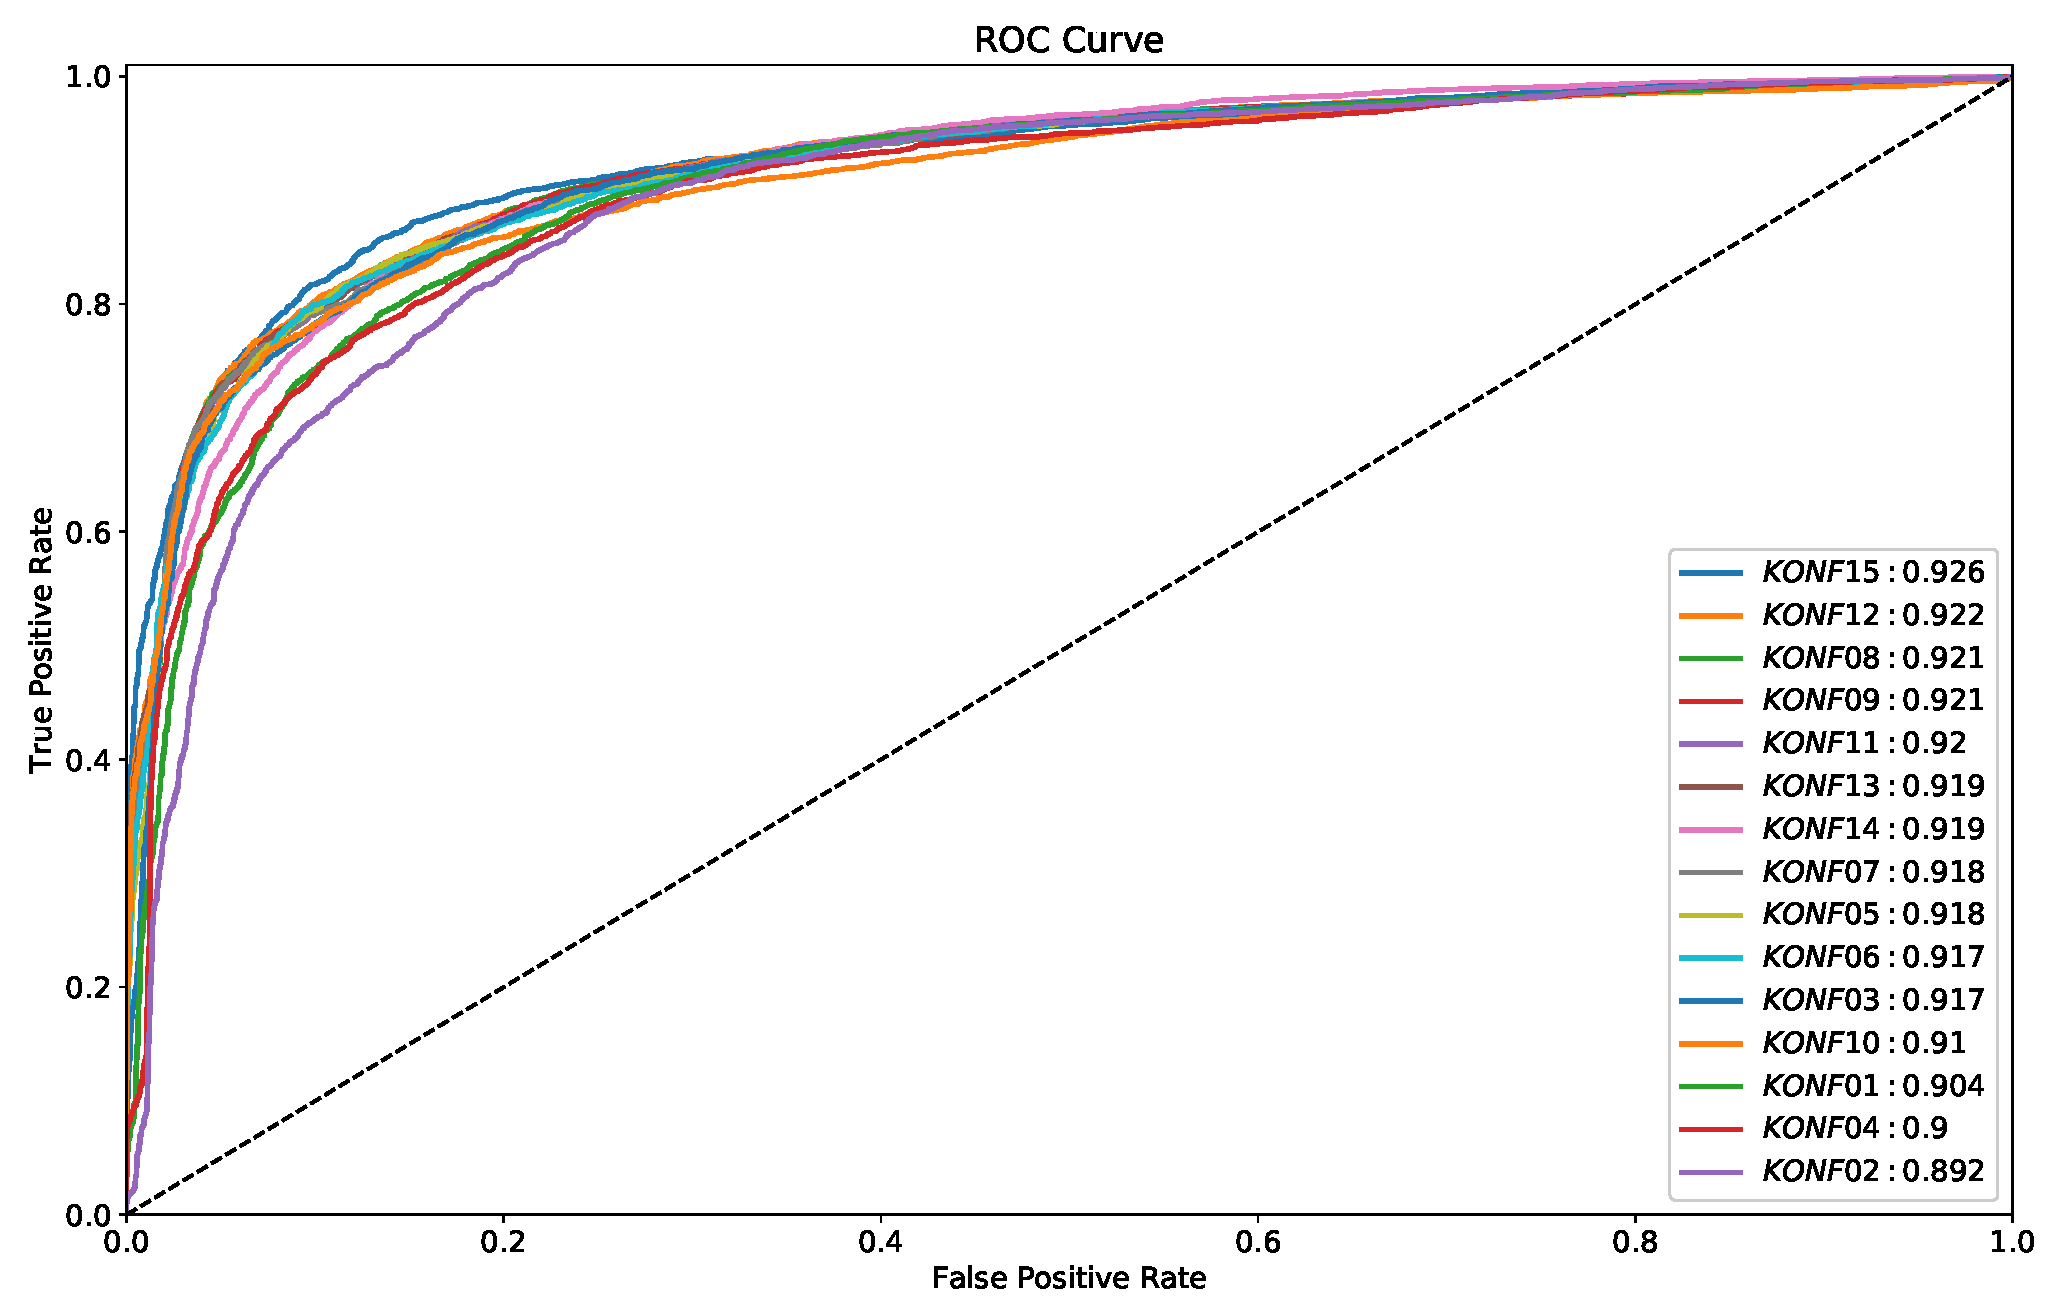
\includegraphics[width=16cm]{figures/roc1}
\caption{ROC křivka natrénovaných klasifikátorů}
\label{fig:rocCurve1}
\end{figure}

\begin{table}[H]
\centering
\caption{Přehled vytrénovaných klasifikátorů a jejich trénovacích parametrů. Parametry $\varepsilon$, kritéria ukončení a počet pozitivních vzorků (5649) byly stejné.}
\begin{tabular} { |c|c|c|c|c|c| }
\hline
{}          & {par. C} & {par. P}    & {max iterací} & {počet neg. vzorků} & {Přesnost \%}  \\ \hline
KONF 01		& 	0.005	& 	  0.02	 &   2000   	 &		  3000   	   &     83	 		\\ \hline
KONF 02		& 	0.005	& 	  0.01	 &   3500   	 &		  3000   	   &     81	 		\\ \hline
KONF 03		& 	0.001	& 	  0.02	 &   2000   	 &		  6000   	   &     83	 		\\ \hline
KONF 04		& 	0.001	& 	  0.02	 &   4500   	 &		  6000   	   &     81	 		\\ \hline
KONF 05		& 	0.005	& 	  0.4 	 &   3500   	 &		  6000   	   &     84	 		\\ \hline
KONF 06		& 	0.01 	& 	  0.4 	 &   3000   	 &		  6000   	   &     84	 		\\ \hline
KONF 07		& 	0.005	& 	  0.01	 &   2500   	 &		  9000   	   &     82	 		\\ \hline
KONF 08		& 	0.005	& 	  0.25	 &   2000   	 &		  9000   	   &     82	 		\\ \hline
KONF 09		& 	0.005	& 	  0.25	 &   3000   	 &		  9000   	   &     82	 		\\ \hline
KONF 10 	& 	0.01 	& 	  0.02	 &   3000   	 &		  9000   	   &     80	 		\\ \hline
KONF 11 	& 	0.01 	& 	  0.25	 &   2000   	 &		  9000   	   &     82	 		\\ \hline
KONF 12 	& 	0.01 	& 	  0.25	 &   2500   	 &		  9000   	   &     82	 		\\ \hline
KONF 13 	& 	0.01 	& 	  0.25	 &   4500   	 &		  9000   	   &     82	 		\\ \hline
KONF 14 	& 	0.5	 	& 	  0.1	 &   1200   	 &		  9000   	   &     81	 		\\ \hline
KONF 15 	& 	0.5		& 	  0.1	 &   2000   	 &		  9000   	   &     83	 		\\ \hline
\end{tabular}
\label{classTab1}
\end{table}

Vybral jsem konfiguraci 15, protože oblast pod křivkou byla největší ze všech natrénovaných, přesnost tohoto klasifikátoru je v tabulce \ref{classTab2}. Výsledky testování ostatních klasifikátorů jsou v příloze této práce. Detekce může nabývat maximálně 4 stavů:
\begin{itemize}
	\item{True Positive (\textbf{TP}) - detektor správně rozpoznal chodce.}
	\item{True Negative (\textbf{TN}) - detektor tuto oblast ignoroval.}
	\item{False Positive (\textbf{FP}) - detektor označil tuto oblast za chodce, ovšem se zde nenachází.}
	\item{False Negative (\textbf{FN}) - v oblasti se vyskytuje chodec avšak byl ignorován.}
\end{itemize}

Díky těmto stavům můžeme vypočítat přesnost detekce:
\begin{equation*}
\centering
 \label{eq:accuracy}
 \begin{aligned}
Accuracy = \frac{TP + TN}{TP + TN + FP + FN}
 \end{aligned}
\end{equation*}

\begin{table}[H]
\centering
\caption{Přesnost konfigurace klasifikátoru číslo 15}
\begin{tabular} { |c|c|c|c|c| }
\hline
{}          & {TP/FN} 	 & {TN/FP} 	& {Přesnost \%} & {AUC}  \\ \hline
KONF 15 	&  3479/1572 & 4912/192 &     83 		& 0.926  \\ \hline
\end{tabular}
\label{classTab2}
\end{table}
Na tento klasifikátor jsem se rozhodl aplikovat algoritmus substrakce pozadí, a tak zefektivnit jeho rychlost a správnost detekce.

\subsection{Aplikace algoritmu Mixtura Gaussiánů}
V předchozí kapitole jsem popsal, jak probíhalo zvolení optimálního klasifikátoru a nyní jej pojďme použít na reálná data. Chodci jsou v použitých videosekvencích a obrázcích anotováni v textových souborech každý zvlášť. První řádek tohoto textového souboru odpovídá počtu snímku videa a další řádky jsou věnovány samotným anotacím, kde první číslo vyjadřuje číslo snímku a následující 4 čísla jsou body dané anotace.

Testovací video je ve 3 druzích rozlišení, základní informace o videosekvencích je uvedena v tabulce \ref{videosTab}, rozdíl mezi výskytem osob a snímků za sekundu je způsobené převodem videa.

\begin{table}[H]
\centering
\caption{Přehled testovaných videozáznamů}
\begin{tabular} { |c|c|c|c|c| }
\hline
{Název videa}   & {Rozlišení} 	& {Počet snímků}    & {FPS} & {Výskyt osob na snímcích}  	\\ \hline
cctv4.mp4 		&  640 x  360	& 781  				& 29,97	& 	754							\\ \hline
cctv4.avi		& 1280 x  720	& 626  				& 24,00	& 	597							\\ \hline
cctv4.mov 		& 1920 x 1080	& 781  				& 29,97	& 	749							\\ \hline
\end{tabular}
\label{videosTab}
\end{table}

Chodci se ve videosekvenci mohli vyskytovat kdekoliv, proto jsem namísto přesnosti počítal F1--skóre. Ke svému výpočtu nepotřebuje true negative, které by bylo nemožné získat z každého snímku z videa. Výpočet F1--skóre je následující:
\begin{equation*}
\centering
 \label{eq:f1score}
 \begin{aligned}
F1-score = \frac{ 2TP}{2TP + FP + FN}
 \end{aligned}
\end{equation*}
Také jsem stanovil pravidlo pro pozitivní detekci a to takové, že výstup z detektoru je považován za pozitivní právě tehdy, když jeho plocha je větší než polovina anotované plochy. 

Navzdory tomu, že tyto počítače podporují rozšíření NEON a obě knihovny byly kompilovány s tímto rozšířením, výsledky nebyly až tak časově uspokojivé jak jsem očekával. V následujících tabulkách jsou uvedeny výsledky detekce mého vytrénovaného detektoru včetně původního detektoru lidí, který je obsažen v OpenCV (v tabulkách je zaznamenán jako ``default'').
V tabulkách \ref{resultTabIMX}, \ref{resultTabRPI3} a \ref{resultTabBPI} jsou uvedeny výsledky detekce z každého videa na jednotlivém zařízení. Tabulka \ref{resultTabDesktop} jsou výsledky z desktopového počítače.  
\begin{table}[H]
\catcode`\-=12
\centering
\caption{Výsledky detekce počítače HummingBoard Pro i.MX6 }
\label{resultTabIMX}
\begin{tabular}{|c|c|c|c|c|c|c|c|}
\hline
                         & Typ algoritmu   	& ALG FPS & Délka detekce & TP & FN & FP & F1--skóre \\ \hline
\multirow{6}{*}{cctv4.mp4} & HOG        	&         &               &    &    &    &          \\ \cline{2-8} 
                         & HOG + MOG  		&         &               &    &    &    &          \\ \cline{2-8}  
                         & FHOG       		&         &               &    &    &    &          \\ \cline{2-8}  
                         & FHOG + MOG 		&         &               &    &    &    &          \\ \cline{2-8}  
                         & default	 		&         &               &    &    &    &          \\ \cline{2-8}  
                         & default + MOG	&         &               &    &    &    &          \\ \hline\hline 
\multirow{6}{*}{cctv4.avi} & HOG        	&         &               &    &    &    &          \\ \cline{2-8} 
                         & HOG + MOG  		&         &               &    &    &    &          \\ \cline{2-8}  
                         & FHOG       		&         &               &    &    &    &          \\ \cline{2-8} 
                         & FHOG + MOG 		&         &               &    &    &    &          \\ \cline{2-8} 
                         &  default 		&         &               &    &    &    &          \\ \cline{2-8}  
                         & default + MOG	&         &               &    &    &    &          \\ \hline \hline
\multirow{6}{*}{cctv4.mov} & HOG        	&         &               &    &    &    &          \\ \cline{2-8} 
                         & HOG + MOG  		&         &               &    &    &    &          \\ \cline{2-8} 
                         & FHOG       		&         &               &    &    &    &          \\ \cline{2-8}  
                         & FHOG + MOG 		&         &               &    &    &    &          \\ \cline{2-8} 
                         & default 		 	&         &               &    &    &    &          \\ \cline{2-8} 
                         & default + MOG 	&         &               &    &    &    &          \\ \hline
\end{tabular}
\end{table}


\begin{table}[H]
\catcode`\-=12
\centering
\caption{Výsledky detekce počítače Raspberry PI3}
\label{resultTabRPI3}
\begin{tabular}{|c|c|c|c|c|c|c|c|}
\hline
                         & Typ algoritmu 	& ALG FPS & Délka detekce [s] & TP 		& FN 	& FP 	& F1--skóre [\%] \\ \hline
\multirow{6}{*}{cctv4.mp4} & HOG         	&   0,95  &   826,7       	  & 441   	& 313   & 158   &   65      	\\ \cline{2-8} 
                         & HOG + MOG  		&   3,89  &   200,7       	  & 579		& 175  	& 18   	& 	86	        \\ \cline{2-8} 
                         & FHOG       		&         &   			  &    		&    	&    	& 		        \\ \cline{2-8} 
                         & FHOG + MOG 		&         &               	  &    		&    	&    	& 		        \\ \cline{2-8} 
                         & default	 		&         &               	  &    		&    	&    	& 		        \\ \cline{2-8} 
                         & default + MOG 	&               	  &    		&    	&    	& 		&        \\ \hline\hline 
\multirow{6}{*}{cctv4.avi} & HOG      		&   0,65  &   963,5        	  & 416   	& 181 	& 13    & 	81	        \\ \cline{2-8} 
                       & HOG + MOG  		&   1,48  &   524,5       	  & 470		& 127 	& 20   	& 	86	        \\ \cline{2-8} 
                         & FHOG       		&         &               	  &    		&    	&    	& 		        \\ \cline{2-8} 
                         & FHOG + MOG 		&         &               	  &    		&    	&    	& 		        \\ \cline{2-8} 
                         & default	 		&         &               	  &    		&    	&    	& 		        \\ \cline{2-8} 
                         & default + MOG 	&         &               	  &    		&    	&    	& 		        \\ \hline \hline
\multirow{6}{*}{cctv4.mov} & HOG      		&   0,35  &   2 217,1      	  & 572 	& 177 	& 114  	& 	80	        \\ \cline{2-8} 
                         & HOG + MOG  		&   0,38  &   2 080,6      	  & 543		& 206  	& 66	& 	80	        \\ \cline{2-8} 
                         & FHOG       		&         &               	  &    		&    	&    	& 		        \\ \cline{2-8} 
                         & FHOG + MOG 		&         &               	  &    		&    	&    	& 		        \\ \cline{2-8} 
                         & default	 		&         &               	  &    		&    	&    	& 		        \\ \cline{2-8} 
                         & default + MOG 	&         &               	  &    		&    	&    	& 		        \\ \hline
\end{tabular}
\end{table}


\begin{table}[H]
\catcode`\-=12
\centering
\caption{Výsledky detekce počítače Banana PI BPI-M1}
\label{resultTabBPI}
\begin{tabular}{|c|c|c|c|c|c|c|c|}
\hline
                         & Typ algoritmu	& ALG FPS & Délka detekce [s] & TP 	  & FN 	& FP 	& F1--skóre [\%] \\ \hline
\multirow{6}{*}{cctv4.mp4} & HOG      		&  0,44   &   1 795,5    	  & 437   & 317 & 157  	&   65     		\\ \cline{2-8} 
                         & HOG + MOG  		&  2,92   &     267,5     	  & 577   & 177 & 15  	&   86     		\\ \cline{2-8} 
                         & FHOG       		&         &               	  &    &    &    &          \\ \cline{2-8} 
                         & FHOG + MOG 		&         &               	  &    &    &    &          \\ \cline{2-8}  
                         & default	 		&         &               	  &    &    &    &          \\ \cline{2-8}  
                         & default + MOG 	&         &               	  &    &    &    &          \\ \hline\hline 
\multirow{6}{*}{cctv4.avi} & HOG        	&  0,33   &   1 909,3     	  & 416	  & 181  & 13   &   81     		\\ \cline{2-8} 
                         & HOG + MOG  		&  0,85   &     739,4      	  & 470   & 127  & 20   &   86          \\ \cline{2-8} 
                         & FHOG       		&         &               	  &    &    &    &          \\ \cline{2-8} 
                         & FHOG + MOG 		&         &               	  &    &    &    &          \\ \cline{2-8} 
                         & default	 		&         &               	  &    &    &    &          \\ \cline{2-8} 
                         & default + MOG 	&         &               	  &    &    &    &          \\ \hline \hline
\multirow{6}{*}{cctv4.mov} & HOG        	&  0,14   &   5 718,8     	  & 572	  & 177  & 114  &   80		    \\ \cline{2-8} 
                         & HOG + MOG  		&  0,21   &   3 709,5      	  & 544   & 205  & 66   &   80          \\ \cline{2-8} 
                         & FHOG       		&         &               	  &    &    &    &          \\ \cline{2-8} 
                         & FHOG + MOG 		&         &               	  &    &    &    &          \\ \cline{2-8} 
                         & default	 		&         &               	  &    &    &    &          \\ \cline{2-8} 
                         & default + MOG 	&         &               	  &    &    &    &          \\ \hline
\end{tabular}
\end{table}

\begin{table}[H]
\catcode`\-=12
\centering
\caption{Výsledky detekce desktopového počítače}
\label{resultTabDesktop}
\begin{tabular}{|c|c|c|c|c|c|c|c|}
\hline
                         & Typ algoritmu   & ALG FPS & Délka detekce & TP & FN & FP & F1--skóre \\ \hline
\multirow{6}{*}{cctv4.mp4} & HOG        &         &               &    &    &    &          \\ \cline{2-8} 
                         & HOG + MOG  &         &               &    &    &    &          \\ \cline{2-8} 
                         & FHOG       &         &               &    &    &    &          \\ \cline{2-8} 
                         & FHOG + MOG &         &               &    &    &    &          \\ \cline{2-8}  
                         & default	 &         &               &    &    &    &          \\ \cline{2-8} 
                         & default + MOG &         &               &    &    &    &          \\ \hline\hline 
\multirow{6}{*}{cctv4.avi} & HOG        &         &               &    &    &    &          \\ \cline{2-8} 
                         & HOG + MOG  &         &               &    &    &    &          \\ \cline{2-8} 
                         & FHOG       &         &               &    &    &    &          \\ \cline{2-8} 
                         & FHOG + MOG &         &               &    &    &    &          \\ \cline{2-8} 
                         & default  &         &               &    &    &    &          \\ \cline{2-8} 
                         & default + MOG &         &               &    &    &    &          \\ \hline \hline
\multirow{6}{*}{cctv4.mov} & HOG        &         &               &    &    &    &          \\ \cline{2-8} 
                         & HOG + MOG  &         &               &    &    &    &          \\ \cline{2-8} 
                         & FHOG       &         &               &    &    &    &          \\ \cline{2-8} 
                         & FHOG + MOG &         &               &    &    &    &          \\ \cline{2-8} 
                         & default  &         &               &    &    &    &          \\ \cline{2-8} 
                         & default + MOG &         &               &    &    &    &          \\ \hline
\end{tabular}
\end{table}

V následujícím obrázku \ref{fig:rocCurve2} jsou vykresleny ROC křivky všech videí za použití kombinace HoGu a MoGu. Jak může být zřejmé, klasifikátor není až tak spolehlivý na obsah s vysokým rozlišením, na druhou stranu detekci na průměrném rozlišení (720p) je spolehlivější. Natrénoval jsem klasifikátor na vzorcích o velikosti $48x96$ pixelů proto, aby bylo možné detekovat na různých snímcích bez nutnosti zvětšování obsahu.   

\begin{figure}[H]
\centering
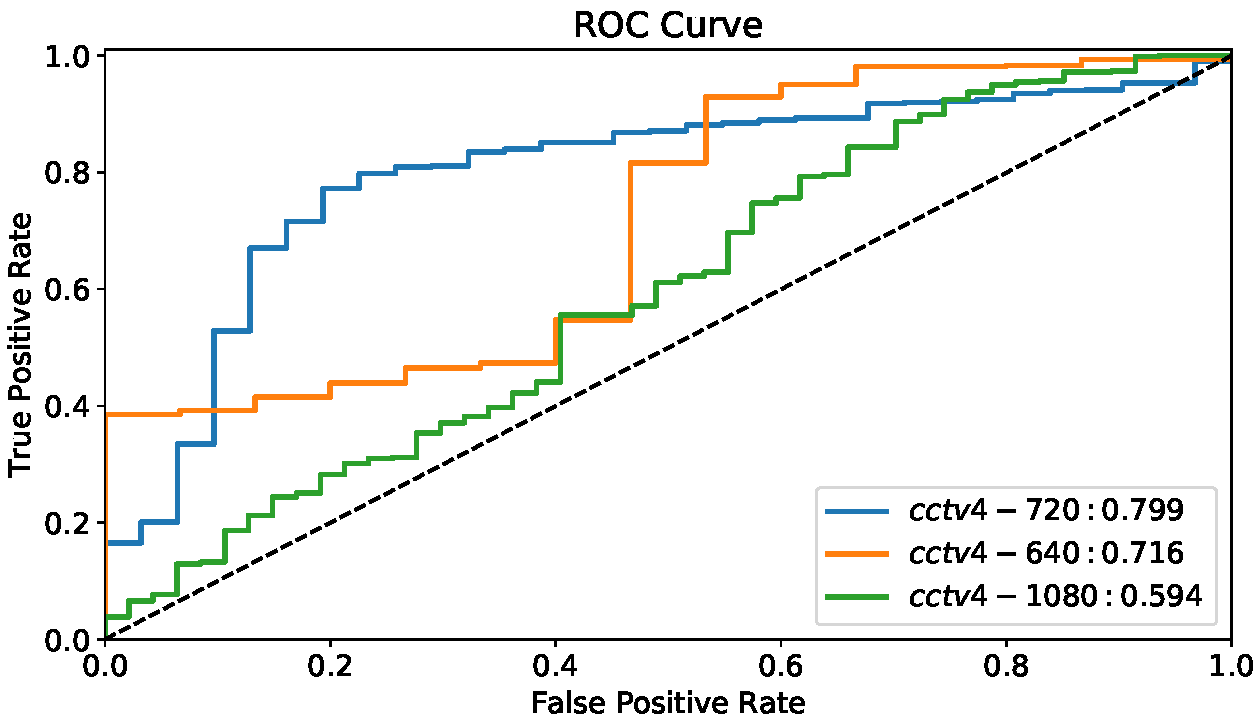
\includegraphics[width=16cm]{figures/roc2}
\caption{ROC křivky klasifikátoru na videosekvencích z tabulky \ref{videosTab}}
\label{fig:rocCurve2}
\end{figure}

Předfiltrování obrazu pomocí subtrakce pozadí se projevilo jako užitečná metodika pro detekci chodců. Nejen, že se zefektivnila detekce odfiltrováním většiny false positive, ale také rychlost samotného algoritmu, například na dvoujádrovém počítači Banana Pi skoro až $7x$ při nízkém rozlišení.  

\section{Závěr}
Dle zadání práce byly otestovány vybrané metodiky z~knihoven OpenCV a~Dlib pro detekci chodců. Z~těchto metodik jsem vybral histogram orientovaných gradientů v~kombinaci s~lineárním klasifikátorem SVM z~OpenCV a~z~knihovny Dlib také histogram orientovaných gradientů. Použití těchto algoritmů obsahuje implementovaná aplikace. Lineární klasifikátor byl zvolen nejen díky své rychlosti klasifikace lineární dělící nadrovinou, ale také proto, že toto jádro je podporováno v~metodě s~posuvným oknem, a~tak nebylo nutné vytvářet vlastní implementaci této detekce, která by jistě nedosahovala tak velkého výpočetního výkonu. 

Při trénování klasifikátoru hrálo důležitou roli správné zvolení trénovací sady a~trénovacích parametrů. Trénovací sada by měla být co nejkvalitnější a~měla by obsahovat co nejméně stínů a~artefaktů. Jak je zmíněno v~textu, aplikace disponuje křížovou validací a~testováním klasifikátoru, které sloužilo ke zvolení co nejvíce optimálních parametrů a~sady tak, abych docílil co nejpřesnějšího a~optimálního klasifikátoru.

Zjistil jsem, že má implementace dané problematiky detekce chodců na embedded zařízeních není dostačující. Na druhou stranu metoda substrakce pozadí značně urychlila detekci, minimálně na jeden snímek za sekundu.

Aplikace by mohla být v~budoucnu obohacena o~vlastní implementaci substrakce pozadí nebo jiným způsobem ořezání výstupního obrazu této substrakce, což by mohlo značně zvýšit výkon aplikace. Dále by práce mohla být rozšířena o~další klasifikátory, například kaskádovými. Tyto kaskádové klasifikátory by značně zvýšily výkon detekce chodců na daných zařízeních a~dosahovaly by většího počtu snímků za sekundu. Dalším možných vývojem je zvolit ARM zařízení s~grafickým jádrem a~implementovat histogram orientovaných gradientům za pomocí technologie Cuda. Také předběžné zpracování obrazu před samotnou detekcí by mohlo být provedeno paralelně.

%Dle zadání práce byly otestované vybrané metodiky z knihoven OpenCV a Dlib pro rozpoznávání chodců. Z těchto metodik byly vybrány algoritmy z OpenCV - Histogram orientovaných gradientů, kaskádové klasifikátory a z Dlib knihovny byl vybrán Histogram orientovaných gradientů a tyto algoritmy byly implementovány v aplikaci. Obě tyto knihovny disponují nástroji pro natrénování klasifikátoru, které se dají poté použít na samotnou detekci.

%Trénování klasifikátoru hraje důležitou roli pro samotnou detekci, protože zvyšuje přesnost detekce a účinnost klasifikátoru.  Další významnou roli na samotnou úspěšnost klasifikátoru je množina trénovacích dat a nastavení trénování klasifikátoru. Tato data by měla být co nejpřesnější a obsahovat minimum stínu a minimum artefaktů. Jak bylo již v tomto dokumentu zmíněno, aplikace obsahuje i nástroje pro otestování klasifikátoru na daných testovacíh datech, které slouží především k přibližnému zvolení parametrů klasifikátoru.

%Tato aplikace by mohla být nadále rozšiřována dalšími klasifikátory pro porovnání rychlosti a výsledkům k již naimplementovaným. 
%
\begin{thebibliography}{99}
	\bibitem{skincolor:obr} \textit{Dostupné z: \url{http://humanorigins.si.edu/sites/default/files/styles/home_slider_phablet/public/KidComp_landscape.jpg}}
	\bibitem{openCV:sklansky}SKLANSKY, Jack. \textit{Finding the convex hull of a simple polygon.} [online] Pattern Recognition Letters, December 1982 . [cit. 11.03.2018].
		\textit{Dostupné z: \url{http://www.sciencedirect.com/science/article/pii/0167865582900162}}
	\bibitem{mog:zivkovic}ZIVKOVIC, Zoran. \textit{Improved adaptive Gausian mixture model for background subtraction.} [online] International Conference Pattern Recognition, UK, August, 2004 [cit. 11.03.2018].
		\textit{Dostupné z: \url{http://www.zoranz.net/Publications/zivkovic2004ICPR.pdf}}
	%\bibitem{edgeTemplate} PAPAGEORGIU Constantine, POGGIO Tomaso A. \textit{A Trainable Pedestrian Detection System} [online] International Journal of Computer Vision (IJCV), November, 2000  [cit. 20.03.2018]. 
 	%	\textit{Dostupné z: \url{https://www.researchgate.net/publication/2467374_A_Trainable_Pedestrian_Detection_System}}
 %	\bibitem{partModels} CHO, Hyunggi, RYBSKI, Paul, BAR-HILLER, Aharon, ZHANG, Wende,  \textit{Real-time pedestrian detection with deformable part models} [online] IEEE, July 05, 2012  [cit. 20.03.2018]. 
 %		\textit{Dostupné z: \url{http://ieeexplore.ieee.org/document/6232264/}}
% 	\bibitem{edgelet} WU, Bo, NEVATIA Ram, \textit{Detection of multiple, partially occluded humans in a single image by Bayesian combination of edgelet part detectors} [online] IEEE, December, 2005 [cit. 20.03.2018]. 
 %		\textit{Dostupné z: \url{http://ieeexplore.ieee.org/document/1541243/}}
 %	\bibitem{orientationFeatures} MIKOLAJCZYK, Krystian, SCHMID, Cordelia, ZISSERMAN, Andrew, \textit{Human detection based on a probabilistic assembly of robust part detectors} [online] ECCV, 2004 [cit. 20.03.2018]. 
% 		\textit{Dostupné z: \url{https://link.springer.com/chapter/10.1007/978-3-540-24670-1_6}}
% 	\bibitem{leibe} LEIBE, Bastian, SEEMANN, Edgar, SCHIELE Bernt, \textit{Pedestrian detection in crowded scenes} [online] IEEE, July 25, 2005 [cit. 20.03.2018]. 
% 		\textit{Dostupné z: \url{http://ieeexplore.ieee.org/document/1467359/}}
% 	\bibitem{motionAlg1} BARNICH, Olivier, JODOGNE, Sébastien, DROOGENBROECK, Marc, Van, \textit{Robust analysis of silhouettes by morphological size distributions} [online] Advanced Concepts for Intelligent Vision Systems(ACIVS), 2006 [cit. 20.03.2018]. 
% 		\textit{Dostupné z: \url{https://link.springer.com/chapter/10.1007/11864349_67}}
% 	\bibitem{motionAlg2} PIÉRARD, Sébastien, LEJEUNE, Anne, DROOGENBROECK, Marc, Van, \textit{A probabilistic pixel-based approach to detect humans in video streams}  [online] IEEE, July 12, 2011  [cit. 20.03.2018]. 
% 		\textit{Dostupné z: \url{http://ieeexplore.ieee.org/document/5946555/}}
% 	\bibitem{multiCameras} FLEURET Francois, BERCLAZ, Jerome, LENGAGNE Richard, FUA, Pascal, \textit{Multi-Camera People Tracking with a Probabilistic Occupancy Map} [online] IEEE, December 18, 2007  [cit. 20.03.2018]. 
 		\textit{Dostupné z: \url{http://ieeexplore.ieee.org/document/4359319/}}
	\bibitem{openCV:MOG}ITSEEZ, Open Source Computer Vision documentation v3.2.0 \textit{How to Use Background Subtraction Methods} [online] Itseez, April, 2014 [cit. 11.03.2018].
		\textit{Dostupné z: \url{http://docs.opencv.org/3.2.0/d1/dc5/tutorial_background_subtraction.html}}
	\bibitem{hog:dalal} {DALAL, Navneet, TRIGGS, Bill. \textit{Histogram of oriented gradients for human detection}. [online] IEEE, July 25, 2005. [cit. 11.03.2018].
		\textit{Dostupné z: \url{https://lear.inrialpes.fr/people/triggs/pubs/Dalal-cvpr05.pdf}}}
	\bibitem{shapeContext} BELONGIE, Serge, MALIK, Jitendra, \textit{Matching with shape contexts}. [online] IEEE, August 06, 2002 [cit. 30.03.2018]. 
 		\textit{Dostupné z: \url{http://ieeexplore.ieee.org/document/853834/}}
 	\bibitem{siftPaper} LOWE, David, \textit{Object recognition from local scale-invariant features}. [online] IEEE, September, 1999 [cit. 30.03.2018]. 
 		\textit{Dostupné z: \url{http://ieeexplore.ieee.org/document/790410/}}
	\bibitem{hog:obr} \textit{Dostupné z: \url{http://www.learnopencv.com/wp-content/uploads/2016/11/hog-cells.png}}
	\bibitem{libsvm} CHANG, Chih-Chung, LIN, Chin-Jen, \textit{LIBSVM: A Library for Support Vector Machines}. [online] ACM Transactions on Intelligent Systems and Technology, 2001 [cit. 31.03.2018]. 
 		\textit{Dostupné z: \url{https://www.csie.ntu.edu.tw/~cjlin/libsvm/}}
	\bibitem{svm:vapnik} VAPNIK, Vladimir, CORTES, Corinna, \textit{Support-vector networks}. [online] Kluwer Academic Publishers, February 20, 1995 [cit. 30.03.2018]. 
 		\textit{Dostupné z: \url{https://link.springer.com/article/10.1007\%2FBF00994018}}
	\bibitem{svmsucc} KOWALCZYK, Alexandre.  \textit{Support Vector Machines Succinctly}.  [online] Syncfusion, Published on October 23, 2017 [cit. 11.03.2018]. 
		\textit{Dostupné z: \url{https://www.syncfusion.com/ebooks/support_vector_machines_succinctly}}
	\bibitem{csvmclass} BOSER, Bernhard, GUYON, Isabelle, VAPNIK, Vladimir, \textit{A training algorithm for optimal margin classifiers}. [online] ACM Press, 1992 [cit. 01.04.2018]. 
 		\textit{Dostupné z: \url{http://citeseerx.ist.psu.edu/viewdoc/summary?doi=10.1.1.21.3818}}
 	\bibitem{nusvmsvrclass} SCHÖLKOPF, Bernhard, SMOLA, Alex, WILLIAMSON, Robert, BARTLETT, Peter, \textit{New support vector algorithms}. [online] MITP, Neural Computation, May 1, 2000 [cit. 01.04.2018]. 
 		\textit{Dostupné z: \url{http://ieeexplore.ieee.org/document/6790203/}}
 	\bibitem{oneclasssvm} SCHÖLKOPF, Bernhard, PLATT, John, SHAWE-TAYLOR, John, SMOLA, Alex, WILLIAMSON, Robert, \textit{Estimating the support of a high-dimensional distribution}. [online] MITP, Neural Computation, July 1, 2001 [cit. 01.04.2018]. 
 		\textit{Dostupné z: \url{http://ieeexplore.ieee.org/document/6790022/}}
 	\bibitem{svrsvm} VAPNIK, Vladimir \textit{Fast training of support vector machines using sequential minimal optimization.}. Wiley, New York, NY, 1998. 
 	\bibitem{haar:like} HOANG, Van-Dung, VAVILIN, Andrey, JO, Kang-Hyun, \textit{Pedestrian detection approach based on modified Haar-like features and AdaBoost}. [online] IEEE, October, 2012 [cit. 31.03.2018]. 
 		\textit{Dostupné z: \url{http://ieeexplore.ieee.org/document/6393256/}}
 	\bibitem{violajones} VIOLA, Paul, JONES, Michael, \textit{Robust real-time face detection}. [online] IEEE, August 07, 2002 [cit. 31.03.2018]. 
 		\textit{Dostupné z: \url{http://ieeexplore.ieee.org/document/937709/}}
 	\bibitem{lbp:texture} HE, Dong-chen, WANG, Li, \textit{Texture Unit, Texture Spectrum, And Texture Analysis}. [online] IEEE, July, 1990 [cit. 02.04.2018]. 
 		\textit{Dostupné z: \url{http://ieeexplore.ieee.org/document/572934/}}
 	\bibitem{lbp:first} OJALA, T, PIETIKAINEN, M, HARWOOD, D, \textit{Performance evaluation of texture measures with classification based on Kullback discrimination of distributions}. [online] ICPR, Proceedings of the 12th IAPR International Conference on Pattern Recognition, 1994 [cit. 02.04.2018]. 
 		\textit{Dostupné z: \url{http://ieeexplore.ieee.org/document/576366/}}
	\bibitem{lbp:orig} AHONEN, Timo, HADID, Abdenour, PIETIKAINEN, Matti, \textit{Face Description with Local Binary Patterns: Application to Face Recognition}. [online] IEEE, October 30, 2006 [cit. 31.03.2018]. 
 		\textit{Dostupné z: \url{http://ieeexplore.ieee.org/document/1717463/}}
 	\bibitem{adaboost} FREUND, Yoav, E. SCHAPIRE, Robert, \textit{A Decision-Theoretic Generalization of On-Line Learning and an Application to Boosting}. [online] Journal of Computer and System Sciences vol. 55, 1997 [cit. 01.04.2018]. 
 		\textit{Dostupné z: \url{https://www.sciencedirect.com/science/article/pii/S002200009791504X}}
 	\bibitem{hoglpb} WANG, Xiaoyu, HAN, Tony X, YAN, Shuicheng, \textit{An HOG-LBP human detector with partial occlusion handling}. [online] IEEE, July 29, 2010 [cit. 31.03.2018]. 
 	\textit{Dostupné z: \url{http://ieeexplore.ieee.org/document/5459207/}}
	\bibitem{fig:mlvsann} \textit{Dostupné z: \url{https://cdn-images-1.medium.com/max/800/1*ZX05x1xYgaVoa4Vn2kKS9g.png}}
	\bibitem{ann} HILTZ, Frederick, \textit{Analog Computer Simulation of a Neural Element}. [online] IEEE, January, 1962 [cit. 16.04.2018]. 
 	\textit{Dostupné z: \url{https://ieeexplore.ieee.org/document/4322944/}}
 	\bibitem{lenet} LE CUN, Yann, JACKEL Lawrence, BOSER Bernhard, DENKER John, GRAF, Hans, GUYON, Isabelle, HENDERSON, William, HOWARD, Richard, HUBBARD, Douglas, \textit{Handwritten digit recognition: applications of neural network chips and automatic learning}. [online] IEEE, November, 1989 [cit. 16.04.2018]. 
 	\textit{Dostupné z: \url{https://ieeexplore.ieee.org/document/41400/}}
 	\bibitem{sudipdas} Dostupné z: \url{https://www.kaggle.com/sudipdas/datasets}
 	\bibitem{inria} Dostupné z: \url{http://pascal.inrialpes.fr/data/human/}
 	\bibitem{eth} Dostupné z: \url{https://data.vision.ee.ethz.ch/cvl/aess/}
 	\bibitem{tudbrussels} Dostupné z: \url{https://www.mpi-inf.mpg.de/departments/computer-vision-and-multimodal-computing/research/people-detection-pose-estimation-and-tracking/multi-cue-onboard-pedestrian-detection/}
 	\bibitem{kitti} Dostupné z: \url{http://www.cvlibs.net/datasets/kitti/eval_object.php}
 	\bibitem{daimler} Dostupné z: \url{http://www.gavrila.net/Datasets/Daimler_Pedestrian_Benchmark_D/Daimler_Mono_Ped__Detection_Be/daimler_mono_ped__detection_be.html}
 	\bibitem{daimlerstereo} Dostupné z: \url{http://www.gavrila.net/Datasets/Daimler_Pedestrian_Benchmark_D/Daimler_Stereo_Ped__Detection_/daimler_stereo_ped__detection_.html}
 	\bibitem{caltech} Dostupné z: \url{http://www.vision.caltech.edu/Image_Datasets/CaltechPedestrians/datasets/USA/}
 	\bibitem{peta} Dostupné z: \url{http://mmlab.ie.cuhk.edu.hk/projects/PETA.html}
 	\bibitem{cuhk} Dostupné z: \url{http://www.ee.cuhk.edu.hk/~xgwang/CUHK_identification.html}
 	\bibitem{} Dostupné z: \url{}
	\bibitem{Banana} SINOVOIP. BANANA PI BPI-M1 single-board computer [online] SINOVOIP CO., LIMITED\& Banana PI team, April, 2014  [cit. 11.03.2018]. 
		\textit{Dostupné z: \url{http://www.banana-pi.com/eacp_view.asp?id=35}}
 
 \bibitem{} AUTOR, \textit{nazev}. [online] Vydavatel [cit. 02.04.2018]. 
 	\textit{Dostupné z: \url{web}}
\end{thebibliography}


\appendix
\section{Ukázky detekce chodců}
\subsection*{Detekce ve videosekvenci s~konfigurací 15}
Testovací video je z~testovací sady \cite{testvideo}.
\begin{figure}[H]
\centering
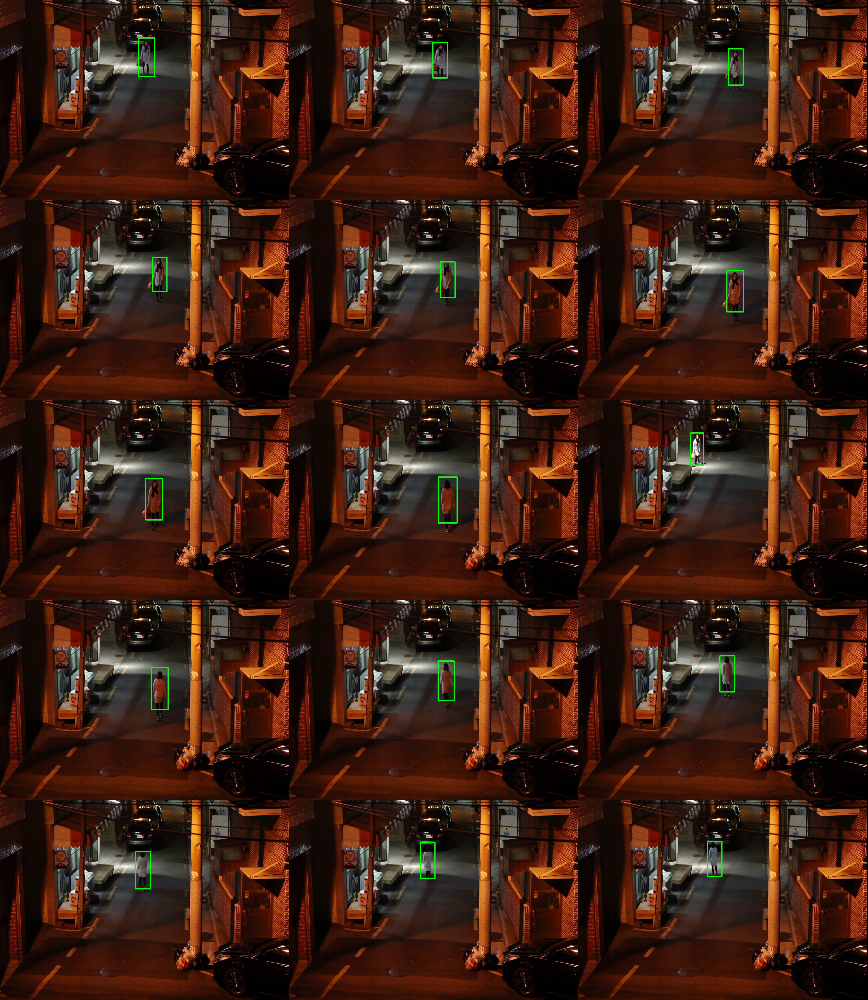
\includegraphics[keepaspectratio,width=16.5cm]{figures/videoMosaic}
\label{appVideo}
\end{figure}
\newpage
\subsection*{Detekce na obrázcích s~konfigurací 15}
Obrázky jsou z~testovací sady \cite{testimg}.
\label{appFigure}
\begin{figure}[H]
\centering
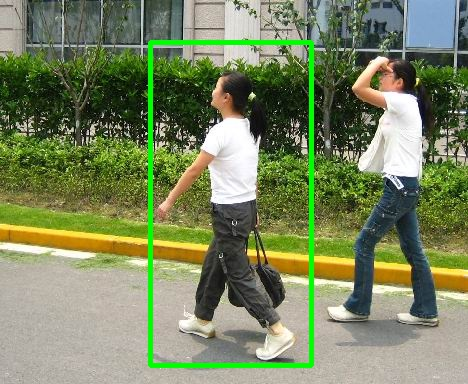
\includegraphics[keepaspectratio, max height=4.5cm,]{figures/ped/d/1}%
\hfill % <-- Seperation
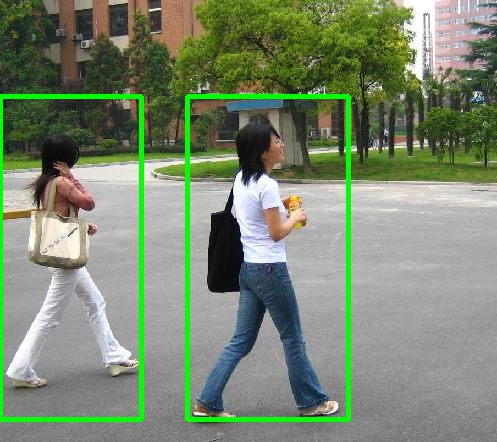
\includegraphics[keepaspectratio, max height=4.5cm,]{figures/ped/d/2}%
\hfill % <-- Seperation
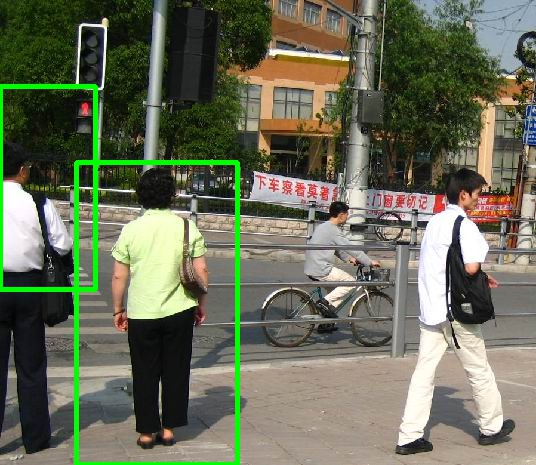
\includegraphics[keepaspectratio, max height=4.5cm,]{figures/ped/d/3}%
\end{figure}

\begin{figure}[H]
\centering
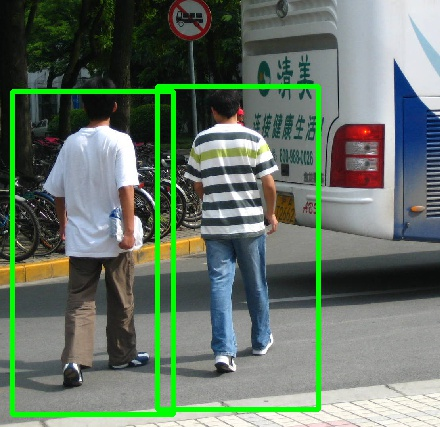
\includegraphics[keepaspectratio, max height=4.5cm,]{figures/ped/d/4}%
\hfill % <-- Seperation
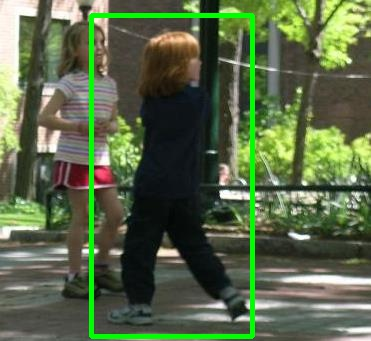
\includegraphics[keepaspectratio, max height=4.5cm,]{figures/ped/d/5}%
\hfill % <-- Seperation
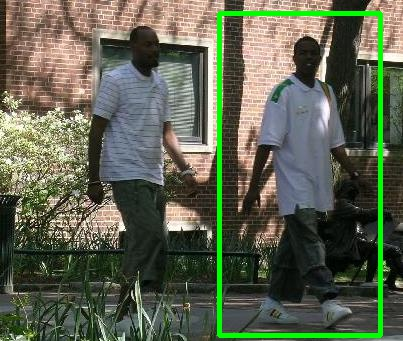
\includegraphics[keepaspectratio, max height=4.5cm,]{figures/ped/d/6}%
\end{figure}

\begin{figure}[H]
\centering
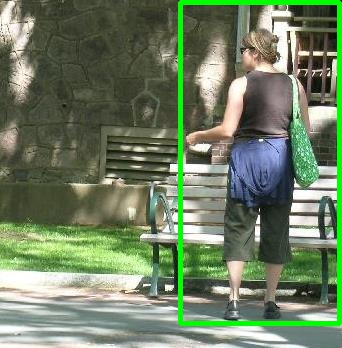
\includegraphics[keepaspectratio, max height=4.5cm,]{figures/ped/d/7}%
\hfill % <-- Seperation
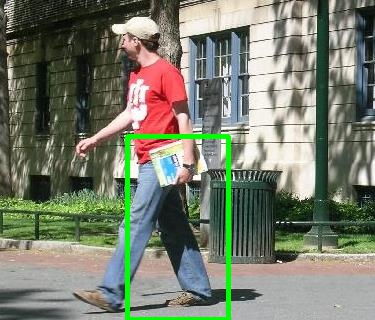
\includegraphics[keepaspectratio, max height=4.5cm,]{figures/ped/d/8}%
\hfill % <-- Seperation
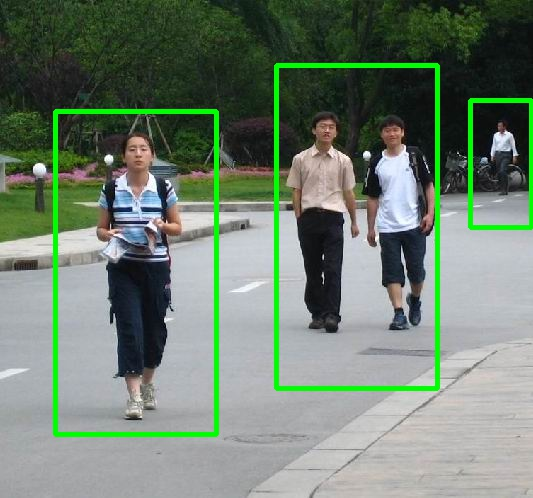
\includegraphics[keepaspectratio, max height=4.5cm,]{figures/ped/d/9}%
\end{figure}

\begin{figure}[H]
\centering
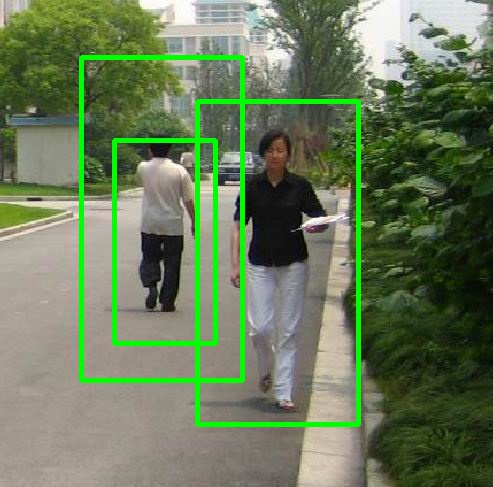
\includegraphics[keepaspectratio, max height=4.5cm,]{figures/ped/d/10}%
\hfill % <-- Seperation
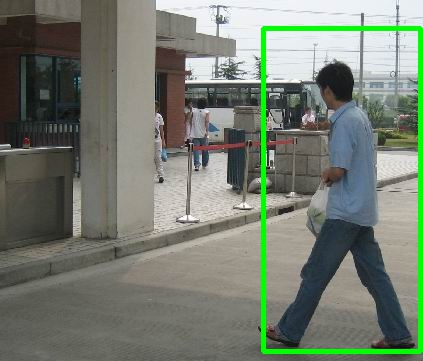
\includegraphics[keepaspectratio, max height=4.5cm,]{figures/ped/d/11}%
\hfill % <-- Seperation
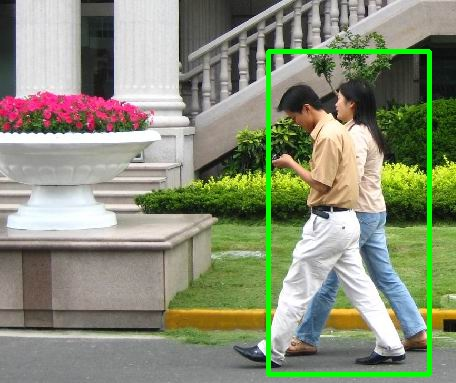
\includegraphics[keepaspectratio, max height=4.5cm,]{figures/ped/d/12}%
\end{figure}

\newpage
\section{Obsah přiloženého CD}
\subsubsection*{Struktura adresáře}
\dirtree{%
.0 project.
.1 apps.
.1 data.
.2 settings.
.2 tested.
.2 trained.
.1 docs.
.1 exDataset.
.1 samples.
.2 negative.
.2 positive.
.1 source.
.1 video.
}
\hfill \break
Součastí jsou i vytrénované klasifikátory z knihovny OpenCV (KONF\_15.yml) a Dlib (pedDet.svm).
\paragraph*{Apps}
Ve složce apps jsou umístěné skripty pro generování ROC křivek, textové soubory s~pravděpodobnostním zařazením a~výsledky křížové validace, resp. testování klasifikátoru. 
\paragraph*{Data}
Zde se nacházejí soubory s~nastavením, anotační soubory videí a~obrázků a~složku tested, kde se ukládá výstup detektoru.
\paragraph*{Docs}
Zde je umístěna programátorská dokumentace. Spouštění se provádí skrze soubor s~názvem index.html.
\paragraph*{ExDataset}
Zde jsou ukázky použitých datasetů.
\paragraph*{Samples}
Zde jsou soubory s~cestami k~negativním a~pozitivním vzorkům.
\paragraph*{Source}
Zde se nachází zdrojový kód implementované aplikace.
\paragraph*{Video}
Zde jsou umístěné videosekvence určené k~testování.

\subsection*{Uživatelská příručka}
\label{manual}
Stručnou nápovědu k~této aplikaci také získáme spuštěním s~argumentem \textbf{-h} nebo \textbf{-help}.
\subsubsection*{Spuštění detekce}
Aplikace dokáže detekovat ze tří druhů zdrojů, z~videa, obrázků a~webové kamery. Detekce ve videosekvenci se spustí argumentem \textbf{-v=<cesta-k-souboru>}, detekce z~webové kamery \textbf{-c=<číslo-zařízení>} a~z~obrázků \textbf{-i=<cesta-k-souboru-s-obrázky>}. Spuštění detekce s~vlastním detektorem vyžaduje další argumenty a~to \textbf{-class=<cesta-ke-klasifikátoru>} a~pro soubor s~jeho nastavením \textbf{-st=<cesta-k-souboru>}. Argumentem \textbf{-viz=1} povolíme náhled detekce.  Například spuštění detekce může vypadat takto: 
\begin{center}
\verb|./Pedestrian -v=video/cctv4_640.mp4 -class=KONF_15.yml| 
\verb|-settings=data/settings/settings_640.txt -viz=1|
\end{center}
\subsubsection*{Trénování klasifikátoru}
Trénování spustíme argumentem \textbf{-type=train}. Po spuštění aplikace s~tímto argumentem bude uživatel vyzván, aby vybral typ trénování. Nastavení pro trénování se nachází externě mimo program v~souboru. Pokud aplikaci nespustíme s~argumentem \textbf{-st=<cesta-k-souboru>}, načte se nastavení z~výchozího souboru \textit{settings.txt}. Argumentem \textbf{-verbose=1} vytiskneme aktuální nastavení trénovacích parametrů před trénovacím procesem.
\subsubsection*{Testování, křížová validace klasifikátoru}
Aplikace také disponuje testováním a~křížovou validací klasifikátoru, tu spustíme argumentem \textbf{-type=test}. Uživatel následně je vyzván k~výberu testování. Aplikace zvládá křížovou validaci klasifikátorů z~knihovny OpenCV i~z~knihovny Dlib. Pro testování nabídne pouze klasikátor z~knihovny OpenCV. 
\subsubsection*{}
\subsubsection*{Tvorba negativních vzorků}
Nástroj se spouští argumentem \textbf{-cs=<cesta-k-souboru-se-snímky>}. Po spuštění začne okamžitě pracovat. Snímky ukládá do složky \uv{makedSamples} a~po dokončení vypíše do konzole dobu trvání procesu. Velikost okna se definuje v~externím souboru nastavení, pokud chceme definovat velikost řezu, musíme nástroj spustis společně s~\textbf{-st=<cesta-k-souboru>}.
\subsubsection*{Anotační nástoj}
Nástroj se spouští argumentem \textbf{-e=<název-videa>}, po spuštění je uživatel dotázán, kolik osob bude anotovat (nanejvýš lze až 5 osob).
Klávesami `0' až `4' se přepíná mezi anotacemi, přičemž se tato selekce vypíše pro kontrolu do konzole. Klávesa `r' slouží pro vynulování vybrané anotace. Klávesou `n' přeskočíme aktuální snímek bez uložení anotovaných pozic. Klávesa `s' uloží aktuální anotované pozice do paměti a~přepne se na další snímek, přičemž pozice první anotace zůstane nezměněná, to umožňuje jednodušší práci, pokud se v~obraze nachází pouze jeden chodec. Klávesy `i', `j', `k' a~`l' umožňuje pohyb v~obraze, pro přesnější umístění anotované části. Pokud tyto klávesy stiskneme společně s~klávesou `shift', umožní nám to měnit velikost aktuálně vybrané anotace. Klávesa `x' uloží aktuální pozice anotací v~paměti do souboru. Tato funkcionalita umožňuje přerušovanou práci na anotacích videosekvence, ale vyžaduje manuální úpravu souboru uživatelem. Po posledním snímku z~videa se nástroj ukončí a~soubor s~anotacemi se uloží na disk se stejným názvem jako bylo zpracovávané video. Soubor je kompatibilní s~jakýmkoliv textovým editorem.
\end{document}